\documentclass[pdflatex,sn-mathphys-num]{sn-jnl}

\usepackage{lineno,hyperref}
\modulolinenumbers[5]
\usepackage{booktabs}
\usepackage{xcolor}
\usepackage{amsfonts}
\usepackage{subcaption}
\usepackage{amsmath}
\usepackage{multirow}
\usepackage{rotating}
\usepackage{float}
\usepackage{subcaption}
% \usepackage[table,xcdraw]{xcolor}
% \usepackage[labelformat=simple]{subfig}
% \renewcommand\thesubfigure{\normalfont(\textbf{\alph{subfigure}})}

\newcommand \pn {UDACM}
\newcommand\tab[1][1cm]{\hspace*{#1}}
\newcommand{\donotadd}[1]{}
%%%%%%%%%%%%%%%%%%%%%%%
%% Elsevier bibliography styles
%%%%%%%%%%%%%%%%%%%%%%%
%% To change the style, put a % in front of the second line of the current style and
%% remove the % from the second line of the style you would like to use.
%%%%%%%%%%%%%%%%%%%%%%%

%% Numbered
%\bibliographystyle{model1-num-names}

%% Numbered without titles
%\bibliographystyle{model1a-num-names}

%% Harvard
%\bibliographystyle{model2-names.bst}\biboptions{authoryear}

%% Vancouver numbered
%\usepackage{numcompress}\bibliographystyle{model3-num-names}

%% Vancouver name/year
%\usepackage{numcompress}\bibliographystyle{model4-names}\biboptions{authoryear}

%% APA style
%\bibliographystyle{model5-names}\biboptions{authoryear}

%% AMA style
%\usepackage{numcompress}\bibliographystyle{model6-num-names}

%% `Elsevier LaTeX' style
%%%%%%%%%%%%%%%%%%%%%%%

\begin{document}

\title[\boldmath$M^2$FA-Net]{\textbf{\boldmath$M^2$FA-Net: A Multimodal Multi-Level Fusion Attention Network for Weed Segmentation}}

\author*[1]{\fnm{Rakesh Kumar} \sur{Sanodiya}}
\email{rakesh.s@iitrpr.ac.in}

\author[2]{\fnm{Manan} \sur{Dudeja}}

\author[3]{\fnm{Lekshmi} \sur{R}}

\author*[4]{\fnm{Matloob} \sur{Khushi}}
\email{matloob.khushi@brunel.ac.uk}

\affil[1]{\orgdiv{School of Artificial Intelligence and Data Engineering},
\orgname{Indian Institute of Technology Ropar},
\orgaddress{\city{Rupnagar}, \state{Punjab}, \country{India}}}

\affil[2]{\orgname{Vellore Institute of Technology},
\orgaddress{\city{Chennai}, \country{India}}}

\affil[3]{\orgname{Amrita School of AI, Amrita Vishwa Vidyapeetham},
\orgaddress{\city{Bengaluru}, \country{India}}}

\affil[4]{\orgdiv{Department of Computer Science},
\orgname{Brunel University of London},
\orgaddress{\city{London}, \country{United Kingdom}}}

\abstract{
Accurate weed segmentation is a fundamental requirement for precision agriculture, enabling targeted weed management and reducing excessive herbicide usage. However, reliable discrimination between crops and weeds remains challenging due to strong visual similarity, overlapping vegetation, varying illumination conditions, and complex field backgrounds. In this paper, we propose $M^2$FA-Net, a multimodal multi-level fusion attention network for crop-weed segmentation that effectively integrates RGB imagery, multispectral information, and vegetation indices. The proposed framework employs dual DeepLabV3-ResNet50 backbones to independently extract spatial and spectral features, followed by progressive multi-level feature fusion to capture complementary information across multiple semantic scales. Convolutional Block Attention Modules (CBAM) are incorporated at each fusion stage to enhance discriminative feature learning, while deep supervision provides improved gradient propagation and optimization stability. Furthermore, a composite loss function combining Cross-Entropy, Dice, and Boundary losses is adopted to jointly optimize pixel-level classification, region overlap, and boundary accuracy. Extensive experiments conducted on the WeedyRice-RGBMS-DB dataset demonstrate the effectiveness of the proposed framework. $M^2$FA-Net achieves a test Intersection over Union (IoU) of 80.79\% and Dice score of 89.21\%, outperforming eleven state-of-the-art CNN-based, transformer-based, and hybrid segmentation models. Ablation studies and hyperparameter sensitivity analyses further validate the contribution of each architectural component and confirm the robustness of the proposed approach. The results demonstrate that $M^2$FA-Net provides an effective and reliable solution for accurate crop--weed segmentation in UAV-based precision agriculture applications.
}
\keywords{Crop-weed segmentation, Precision agriculture, Multi-spectral imaging, Multi level fusion, CBAM, Deep supervision, Semantic segmentation, UAV imagery, Vegetation indices}
\maketitle

\section{Introduction}
\begin{figure}[t]
    \centering
    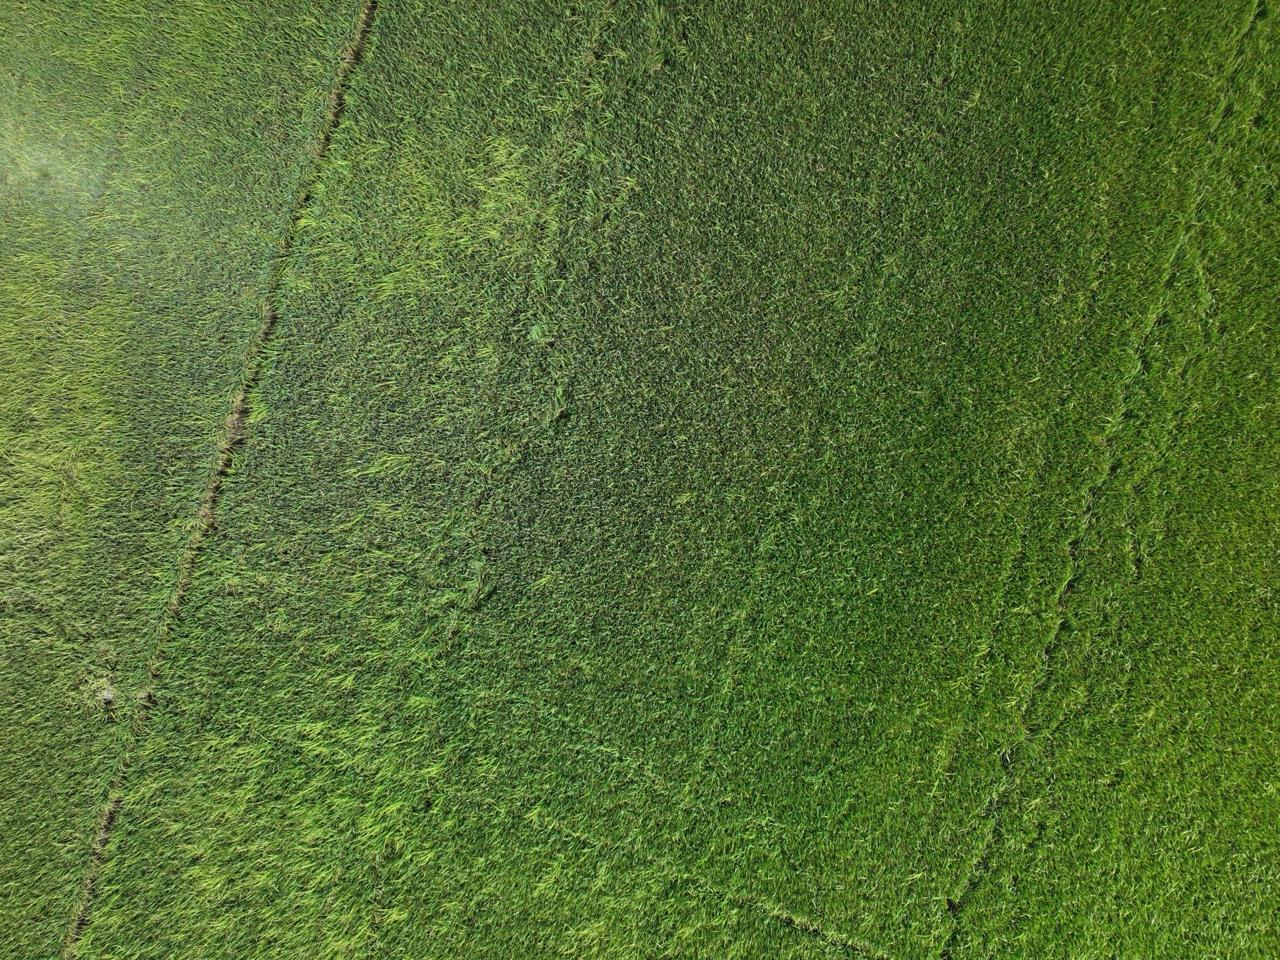
\includegraphics[width=10cm]{Images/sample.JPG}
    \caption{Sample of RGB field image from the dataset showing the visual similarity and overlap between crops and weeds, highlighting the importance of accurate crop-weed segmentation in precision agriculture.}
    \label{fig:sample}
\end{figure}
The global population is growing at an unprecedented rate and is estimated to reach nearly 9 billion by 2050, resulting in a significantly increased demand for food, feed, fiber, and fuel. This situation creates the need for a substantial increase in agricultural productivity \cite{fao2017future}. However, modern agriculture faces many challenges, including decreasing arable land, climate change, and the growing problem of weeds. As a result, significant losses occur in crop production, and weeds can reduce the productivity of crops by 25\%. This means effective weed management is an important component of sustainable agriculture. This problem becomes more serious in rice fields as weedy rice is morphologically very similar to conventionally cultivated rice during the early growth stages, making it difficult to distinguish. As illustrated in Fig.~\ref{fig:sample}, even visual inspection of field images often makes it challenging to clearly distinguish crops from weeds due to overlapping vegetation, similar texture, and comparable color appearance. This morphological similarity makes visual identification difficult and labor-intensive, which often results in delays in intervention or reduced effectiveness\cite{weedy_rice_review}\cite{shahi2023weed}. Conventional weed management methods, such as manual inspection and uniform herbicide spraying, are not only inefficient but also unsustainable from an environmental perspective due to increased chemical usage.



To tackle these issues, precision agriculture is increasingly using unmanned aerial vehicles (UAVs) alongside deep learning methods for the automated differentiation of crops and weeds. Imaging via UAVs allows for the capture of high-resolution images of agricultural fields, offering detailed spatial data crucial for identifying weeds at an early stage \cite{zhao2025deep,saini2025review,pena2013weedmapping,sa2018weednet,bah2018weed,fan2023crossmodal_weed}. In this context, models based on Convolutional Neural Networks (CNNs), including \textit{YOLO}\cite{yaseen2025yolov8}, \textit{Mask R-CNN} \cite{he2017maskrcnn}, \textit{U-Net}\cite{ronneberger2015unet}, \textit{SegNet} \cite{badrinarayanan2017segnet}, and \textit{DeepLab}\cite{chen2017deeplabv3}\cite{chen2018Deeplabv3plus}, have shown excellent results in tasks involving semantic segmentation. For instance, Silva et al. \cite{silva2024deep} presented a comparison among different variants of YOLO, U-Net, and Mask R-CNN, where YOLOv8s achieved more than 99.7\% precision on publicly available aerial images of soybeans and beans.

CNNs have demonstrated good performance in segmentation tasks by exploiting local spatial features, but they still face challenges in complex scenarios, such as agricultural crop-weed segmentation. This is because they cannot effectively model the long-range contextual dependencies that are crucial in complex agricultural scenes. To address this challenge, attention-based approaches, such as the Convolutional Block Attention Module (CBAM), have emerged as effective solutions \cite{woo2018cbam,hu2018senet,oktay2018attentionunet,wang2018nonlocal}. These mechanisms allow the models to learn long-range dependencies and improve the extraction of global contextual information. For instance, Li et al.\cite{li2025improved} have shown 3.08\% improvement on  UNet architecture by leveraging attention mechanisms on the sugar beet dataset. Besides, Transformer-based methods  \cite{dosovitskiy2021vit, xie2021segformer, liu2021swin} are proposed to further improve the modeling of global context. However, the application of these methods in real-time UAV-based applications is still hampered by two main limitations, namely, the requirement of large-scale training datasets and the high computational complexity. For instance, Jiang et al.\cite{jiang2022transformer} explore different variants of transformer on their in-house weed datasets and report that SegFormer achieves the best mIoU 65.74\% compared to all other variants, ie Swin Transformer.
Another important trend in crop–weed segmentation is the fusion of vegetation indices \cite{hunt2013vegetation} and multispectral imaging \cite{zhang2021multispectral} with RGB data. Multispectral images provide additional spectral information about plant physiology, while vegetation indices characterize features such as chlorophyll content and vegetation vigor that are important for enhancing the separability of crops from weeds. Ma et al. \cite{ma2024vegetation_dl} have shown that the integration of these modalities into deep learning frameworks could improve the segmentation performance. However, most existing methods use simple early fusion strategies, which cannot effectively solve the distribution shift problem from heterogeneous data modalities. 

To address these limitations, we propose \textbf{$\mathbf{M^2}$FA-Net}, a Multi-Level Multimodal Fusion framework for crop-weed segmentation.
The proposed method performs hierarchical feature fusion at multiple progressive encoder levels, enabling the model to capture complementary cross-modal cues at multiple spatial resolutions and
abstraction levels. CBAM attention modules are applied after each fusion level to selectively recalibrate the integrated
features. Deep supervision via auxiliary classifiers provides rich intermediate gradient signals, and a composite loss
function jointly optimizes pixel accuracy, region overlap, and boundary sharpness. The main contributions of this work are summarized as follows:
\begin{itemize}
\item Proposed a dual-branch DeeplabV3 architecture pretrained on ResNet50 that fuses RGB and multispectral features at multiple hierarchical encoder levels, enabling adaptive integration of complementary cross-modal information across all spatial resolutions.
\item Integrated CBAM attention modules at each fusion stage to selectively emphasize discriminative channel and spatial features, suppressing background noise and improving cross-modal feature quality at every level of abstraction.
\item Introduced a deep supervision mechanism via multiple auxiliary segmentation classifiers attached to intermediate fusion stages, providing dense gradient flow to all backbone layers and substantially improving convergence and final segmentation performance
\item Adopted a composite loss function that combines cross-entropy, Dice, and boundary-sensitive loss terms, jointly optimizing pixel-level accuracy, region overlap, and boundary sharpness for challenging crop--weed segmentation.
\item Experimented on the WeedyRice-RGBMS-DB dataset and achieved best performance among the evaluated methods, with a test IoU of 80.79\% and a Dice score of 89.21\%, surpassing eleven competitive baseline models.

% Systematic ablation studies validate the contribution of each component.
\end{itemize}
\section{Related Works}
Agricultural image analysis has made remarkable progress with the rise of deep learning, enhancing crop monitoring, disease diagnosis, weed detection, and semantic segmentation tasks significantly \cite{lei2024segmentationreview}. We are moving away from handcrafted feature-based methods that have been widely used in previous studies, as such approaches often fail in real-world conditions with illumination variation, occlusion, and complex backgrounds. Weed detection and segmentation remain particularly challenging tasks due to the visual similarities between crops and weeds, varying lighting conditions, and different soil backgrounds \cite{zhao2025deep,saini2025review}. Over time, researchers have explored a wide spectrum of strategies, ranging from convolutional networks to attention-enhanced models and transformer-based frameworks, as well as multimodal data fusion using both RGB and multispectral images, enabling the extraction of vegetation indices such as NDVI and NDRE.

\subsection{CNN-Based Segmentation Approaches}
Convolutional Neural Networks laid the foundation of semantic segmentation in precision agriculture. Encoder-decoder architectures such as U-Net \cite{ronneberger2015unet}, U-Net++ \cite{zhou2018unet++}, PSPNet \cite{zhao2017pyramid}, HRNet \cite{sun2019high}, DenseUNet \cite{safarov2021denseunet}, and DeepLabV3+ \cite{chen2018Deeplabv3plus} have been widely adopted for UAV-based crop monitoring and weed mapping, demonstrating strong ability to capture local spatial patterns and contextual scene information \cite{silva2024deep}. Among these, DeepLabV3+ has drawn attention for its use of atrous convolutions and Atrous Spatial Pyramid Pooling (ASPP), which increase the receptive field with minimal extra computation, making it suitable for dense prediction tasks like weed segmentation\cite{chen2018Deeplabv3plus}. To further improve performance, attention mechanisms such as the Convolutional Block Attention Module (CBAM)\cite{woo2018cbam} have been introduced into CNN pipelines, jointly modeling channel and spatial attention to improve localization accuracy and boundary precision in agricultural scenes\cite{li2022attention_agriculture}. Beyond architectural choices, boundary-aware loss functions and deep supervision strategies have also proven effective in producing improved segmentation outputs, especially where precise plant contour delineation matters for targeted herbicide application. 

\subsection{Transformer-Based Segmentation Approaches}
More recently, transformer-based models have been introduced in the field of agricultural segmentation, which provide a completely different paradigm through global self-attention mechanisms.
Architectures, such as Vision Transformer (ViT) \cite{dosovitskiy2021vit}, SegFormer \cite{xie2021segformer}, Segmenter \cite{strudel2021segmenter}, and Swin Transformer \cite{liu2021swin}, Vision Transformer (ViT) \cite{dosovitskiy2021vit},
Segmenter \cite{strudel2021segmenter},
and Swin Transformer \cite{liu2021swin}
are derived from the transformer architecture introduced by Vaswani et al. \cite{vaswani2017attention}. These have achieved powerful segmentation performance by capturing long-range spatial dependencies that CNNs find intrinsically difficult to capture. This global context awareness is especially helpful in cluttered agricultural scenes where local features alone may not be sufficient to distinguish visually similar plant species. Besides supervised learning paradigms, alternative learning methods for agricultural vision tasks have also been explored in recent research. Kumar et al. \cite{kumar2024zeroshot} proposed a semantic attribute-based zero-shot learning framework for plant disease classification and proved that attribute-guided representations could improve the recognition of unseen disease categories. Such approaches are indicative of the growing curiosity in developing more data-efficient learning methods for agricultural applications. However, a major limitation of pure transformer models is their heavy dependence on large annotated datasets and their high computational requirements, which are practical barriers to real-time deployment in field-based agricultural systems.
\subsection{Hybrid and Multi-modal Fusion Approaches}
Recognizing that CNNs and transformers have complementary strengths, hybrid frameworks have been proposed to combine both of these architectures so that local feature extraction and global contextual modeling can be done together and yield improved segmentation robustness \cite{zhou2018unet++}. Alongside architectural hybridization, multi-modal data fusion has emerged as another direction. RGB imagery alone often falls short under challenging conditions such as changing illumination and background conditions, prompting researchers to integrate multi-spectral bands - particularly Near Infrared (NIR) and Red Edge (RE) — highly correlated with plant physiology \cite{zhang2021multispectral}. Sahin et al. \cite{sahin2023segmentation} fused RGB and multispectral inputs within a CRF-enhanced U-Net framework and reported meaningful segmentation gains on sunflower weed datasets, while Ma et al. \cite{ma2024vegetation_dl} showed that adding vegetation indices to multispectral data improves robustness under different field conditions. But most of the current fusion strategies are based on simple early concatenation at the input level \cite{li2022attention_agriculture}, \cite{yang2025rshrnet}, which does not preserve modality-specific features or robustly align heterogeneous spectral and spatial distributions. Multi-level hierarchical fusion of RGB and multispectral representations is an under-explored topic in agricultural semantic segmentation \cite{li2023weed}, which is directly addressed by the present work. 


Although recent studies have reported improved crop-weed segmentation performance using modified encoder-decoder and ensemble architectures \cite{ganapathy2025cropweed}, most approaches remain dependent on RGB imagery and do not fully exploit complementary multispectral information. Despite progress in these areas, several challenges remain unresolved. Most CNN-based algorithms rely only on RGB imagery and do not benefit from the full range of spectral information available with multispectral sensors. Transformer-based approaches, while powerful in modeling global context, demand substantial annotated data and computational resources that are often impractical in real agricultural deployment scenarios. Hybrid fusion methods have made strides in combining spatial and spectral modalities, yet they predominantly employ simplistic early fusion strategies that fail to capture the complementary nature of heterogeneous data streams at multiple representational levels. Furthermore, relatively few studies have brought together vegetation indices, hierarchical multimodal feature fusion, lightweight attention mechanisms, deep supervision, and boundary-aware optimization within a single cohesive segmentation framework. These collective gaps motivate the present work, which proposes a multi-level fusion DeepLab-based architecture integrating dual-stream ResNet50 backbones, CBAM attention, and a composite loss function designed to deliver accurate and robust weed segmentation under complex, real-world agricultural conditions.

\begin{figure*}[t]
\centering
\includegraphics[width=\linewidth]{Images/MNet_architecture.png}
\caption{Architecture of the proposed framework for multi-modal weed segmentation. RGB and multispectral features are extracted using dual DeepLabV3-ResNet50 backbones and progressively fused at multiple encoder levels. CBAM modules refine the fused features, while auxiliary classifiers provide deep supervision. The final segmentation output is generated through the main classifier head, followed by bilinear upsampling.}
\label{fig:mnet_architecture}
\end{figure*}
\section{Methodology}
% \subsection{Overview}
In this work, we propose $M^2$FA-Net, a multimodal attention-driven semantic segmentation framework for accurate weed segmentation using RGB and multispectral imagery. Figure~\ref{fig:mnet_architecture} shows the proposed architecture and it combines spatial information from RGB images with spectral and vegetation-specific information extracted from multispectral bands and vegetation indices. The overall architecture consists of two parallel DeepLabV3-ResNet50 backbone networks: one processes RGB images while the other processes multispectral inputs containing spectral bands and vegetation indices. Unlike conventional late-fusion approaches that combine modality-specific representations only at the final encoder stage, the proposed method fuses feature maps extracted at different semantic levels progressively using concatenation and 1 × 1 convolution operations, enabling the integration of complementary spectral-spatial cues at every scale of abstraction. At each fusion level, a CBAM attention module recalibrates the fused representation\cite{hu2018senet,wang2018nonlocal}. The final fused representation is passed through a segmentation head to generate dense pixel-wise weed predictions. Additionally, deep supervision and a composite loss function are incorporated to improve optimization stability, gradient flow, and segmentation boundary quality \cite{lee2015dsn}.

\subsection{Input Modalities}
Our framework considers two primary complementary input modalities:
\begin{itemize}
    \item \textbf{RGB Images:} Standard three-channel RGB images that capture spatial structures, texture patterns, and color information.
    \item \textbf{Multispectral Data:} Four spectral bands, namely Green (G), Red (R), Red Edge (RE), and Near-Infrared (NIR), which provide important spectral and physiological information related to vegetation characteristics.
\end{itemize}
To further improve crop-weed discrimination, two vegetation indices are computed from the multispectral bands.
\subsubsection{Normalized Difference Vegetation Index (NDVI)}
NDVI is expressed in the equation ~\ref{eq1}.
\begin{equation}
\text{NDVI} = \frac{NIR - R}{NIR + R}\label{eq1}
\end{equation}
NDVI \cite{rouse1974ndvi} highlights vegetation health by exploiting the strong reflectance of healthy vegetation in the NIR spectrum and absorption in the red spectrum.
\subsubsection{Normalized Difference Red Edge Index (NDRE)}
NDRE is defined in the equation ~\ref{eq2}.
\begin{equation}
\text{NDRE} = \frac{NIR - RE}{NIR + RE}\label{eq2}
\end{equation}
NDRE \cite{gitelson1997chlorophyll} is more sensitive to chlorophyll concentration and plant stress, making it highly effective for precision agriculture applications. Consequently, the multispectral representation is extended into a six-channel input consisting of \{G, R, RE, NIR, NDVI, NDRE\}. Per-channel mean and standard deviation statistics are computed over the training set and used to normalize the multispectral input using Z-scores. This multi-modal representation provides complementary spatial, spectral, and vegetation-specific information for robust weed segmentation.

\subsection{Network Architecture}
$M^2$FA-Net adopts a dual-stream multi-level fusion strategy based on DeepLabV3 with ResNet50 backbones. The architecture is specifically designed to preserve modality-specific characteristics while reliably integrating spatial and spectral information.
\subsubsection{Dual branch Backbone}
Two independent DeepLabV3-ResNet50 encoders pretrained on the COCO-with-VOC-labels benchmark are employed:
\begin{itemize}
    \item \textbf{RGB Encoder:} Processes the three-channel RGB image.
    \item \textbf{Multispectral Encoder:} Processes the six-channel multispectral input containing spectral bands and vegetation indices.
\end{itemize}
At each stage $i$, the encoder outputs feature maps characterized by progressively higher channel dimensions and proportionally lower spatial resolutions.  Since DeepLabV3 is originally designed to accept 3-channel input, the RGB branch processes the 3-channel input without modification, whereas the first convolutional layer of the multispectral backbone is modified to accept six input channels. The additional channels are initialized using the mean of pretrained RGB weights, allowing the model to preserve transfer learning benefits while adapting to multispectral data.
\subsubsection{Multi-Level Feature Extraction}
Different stages of the encoder extract feature maps that represent various semantic levels:
\begin{itemize}
    \item Low-level features capture edges, textures, and local structures.
    \item Mid-level features capture plant structures and shape information.
    \item High-level features capture semantic representations of crops and weeds.
\end{itemize}
The extracted feature maps from the RGB and multispectral branches are stored independently for hierarchical fusion.
\subsubsection{Multi-Level Feature Fusion}
Rather than restricting fusion to the final layers as seen in traditional late-fusion setups, this framework operates multi-level semantic fusion throughout the network architecture. At each encoder stage, RGB and multispectral feature maps are concatenated along the channel dimension and are given in the equation~\ref{eq3}. 
\begin{equation}
F_{fusion}^{(i)} = \text{Concat}(F_{rgb}^{(i)}, F_{ms}^{(i)})\label{eq3}
\end{equation}
where $F_{rgb}^{(i)}$ and $F_{ms}^{(i)}$ are RGB and multispectral features at the $i^{th}$ encoder level, respectively. After concatenation, a $1\times1$ convolution is applied to reduce dimensionality and learn optimal feature interactions:
\begin{equation}
F_{reduced}^{(i)} = \text{Conv}_{1\times1}(F_{fusion}^{(i)})
\end{equation}
This step integrates diverse spatial and spectral features without increasing the network's channel depth \cite{lin2017fpn}.
\subsubsection{CBAM Attention Module}
To enhance feature representation further, the Convolutional Block Attention Module (CBAM)~\cite{woo2018cbam} is applied to the fused features at each level. CBAM sequentially applies channel attention and spatial attention.
\paragraph{Channel Attention}: This attention identifies the most informative feature channels by learning inter-channel relationships and is expressed by the equation ~\ref{eq5}
\begin{equation}
F_{c}^{(i)} = M_c(F^{(i)}) \otimes F^{(i)}\label{eq5}
\end{equation}
where $M_c$ denotes channel attention and $\otimes$ represents element-wise multiplication.
\paragraph{Spatial Attention}: This attention focuses on important spatial regions within the feature map and is defined in equation ~\ref{eq6}
\begin{equation}
F_{s}^{(i)} = M_s(F_c^{(i)}) \otimes F_c^{(i)}\label{eq6}
\end{equation}
where $M_s$ represents spatial attention.

The final attention-refined representation is given in the equation `\ref{eq8}

\begin{equation}
F_{att}^{(i)} = \text{CBAM}(F_{reduced}^{(i)})\label{eq8}
\end{equation}
The attention mechanism enables the network to suppress irrelevant background information, such as soil and shadows while emphasizing discriminative weed regions.
\subsubsection{Deep Supervision}
To facilitate gradient flow and stabilize training, auxiliary classifiers are attached to intermediate feature levels. These auxiliary outputs provide additional supervision during training and encourage meaningful feature learning at different semantic scales. The $L_{\text{final}}$ is expressed in the equation ~\ref{eq9}
\begin{equation}
L_{\text{final}} = L_{\text{main}} + \lambda \sum_{l=1}^{N} L_{\text{aux}}^{l}\label{eq9}
\end{equation}
where \(L_{\text{main}}\) represents the primary segmentation loss computed from the final output prediction, while \(L_{\text{aux}}^{l}\) denotes the auxiliary losses obtained from intermediate supervision levels. The weighting factor \(\lambda\) controls the contribution of auxiliary losses, and \(N\) represents the total number of supervised intermediate levels in the multi-level architecture.
\subsubsection{Segmentation Head}
The last fused feature representation is passed through a segmentation head consisting of convolution, batch normalization, ReLU activation, and dropout layers. The final prediction layer generates pixel-wise logits corresponding to the weed and background classes. 
The low-resolution segmentation map is upsampled to the original image resolution using bilinear interpolation and expressed in equations ~\ref{eq10}~\ref{eq11}.

\begin{equation}
F_{\text{seg}} = Conv_{1\times1}(Conv_{3\times3}(F_{att}^{(i)}))\label{eq10}
\end{equation}

\begin{equation}
F_{\text{out}} = Upsample(F_{\text{seg}})\label{eq11}
\end{equation}
where $F_{seg}$ represents the predicted segmentation map before upsampling.
\subsection{Loss Function}

The model is trained using a composite loss function combining three complementary terms to improve segmentation quality and boundary precision.

\subsubsection{Cross-Entropy Loss}

Cross-Entropy Loss supervises pixel-wise classification:

\begin{equation}
\mathcal{L}_{CE} = - \sum_{i} y_i \log(\hat{y}_i)
\end{equation}

where $y_i$ and $\hat{y}_i$ represent ground truth and predicted probabilities, respectively.

\subsubsection{Dice Loss}

Dice Loss directly optimizes region overlap between predicted and ground-truth masks:

\begin{equation}
\mathcal{L}_{Dice} = 1 - \frac{2 \sum_{i=1}^{N} (p_i g_i) + \alpha}
{\sum_{i=1}^{N} p_i + \sum_{i=1}^{N} g_i + \alpha}
\end{equation}

where $p_i$ denotes the predicted foreground probability for pixel $i$, $g_i$ represents the corresponding ground-truth binary value, $N$ indicates the total number of pixels, and $\alpha$ is a smoothing factor introduced to prevent division by zero \cite{milletari2016vnet}.
Dice Loss is specifically effective under the conditions of class imbalance, which is commonly observed in weed segmentation datasets.
\subsubsection{Boundary Loss}
To increase the contour sharpness and localization of the boundaries, we introduce a Boundary Loss based on Laplacian edge detection. 
\begin{equation}
E_{p} = \text{Conv}_{\text{Lap}}(P), \qquad
E_{g} = \text{Conv}_{\text{Lap}}(G)
\end{equation}
\begin{equation}
\mathcal{L}_{Boundary} = \frac{1}{N} \sum_{i=1}^{N} \left| E_{p}^{i} - E_{g}^{i} \right|
\end{equation}
where $P$ and $G$ denote the predicted segmentation map and ground truth mask, $E_p$ and $E_g$ represent their corresponding edge maps, and $N$ is the total number of pixels \cite{kervadec2019boundary}.
\subsubsection{Overall Loss}

The primary segmentation loss $\mathcal{L}_{\text{main}}$ is defined in the equation ~\ref{eq12}

\begin{equation}
\mathcal{L}_{main} =
0.4\mathcal{L}_{CE}
+
0.4\mathcal{L}_{Dice}
+
0.2\mathcal{L}_{Boundary}\label{eq12}
\end{equation}
The $\mathcal{L}_{main}$ enables the model to improve classification accuracy, region overlap, and boundary precision simultaneously.
\section{Experiments}
To make the comparisons fair, all the models are implemented in Pytorch and trained under identical experimental settings. The training process for all models used both RGB and multispectral images and was performed on a 13th Gen Intel(R) Core i9-13900K (3.00 GHz) processor, an NVIDIA RTX A5000 GPU with 24 GB memory, 128 GB RAM, 1 TB SSD, and 2 TB HDD. The Software environment was Windows 11 Pro, Python 3.10.20, and CUDA 12.4 for accelerated training. The detailed training hyperparameters and optimization settings are presented in Table~\ref{tab:training_details}. We used the same data split as in Table~\ref{tab:dataset_stats} for training, validation and testing. We conducted a series of experiments on the Weedy-Rice dataset based on a uniform training and testing scheme. Our algorithm is compared against other state-of-the-art models, such as CNN models (U-Net), transformer models (Vision Transformer and SegFormer), as well as the hybrid models (TransUNet, Swin models, and DeepLabV3+). To thoroughly investigate the proposed model, all methods are evaluated under the same conditions and fairly compared with the standard segmentation metrics, including Accuracy, Precision, Recall, IoU, and Dice coefficient. The results are given as the mean ± standard deviation over several runs to evaluate robustness. Moreover, ablation studies and qualitative comparisons were carried out to analyse the contribution of each component of our proposed model.
% \subsection{Training Strategy}
% $M^2$FA-Net framework is optimized using the AdamW optimizer \cite{loshchilov2019adamw} with weight decay regularization. A warmup cosine learning rate schedule \cite{loshchilov2017sgdr} is employed to stabilize early-stage optimization and improve convergence during later epochs. During the warmup phase, the learning rate gradually increases to the base learning rate. Subsequently, cosine annealing progressively reduces the learning rate to achieve smoother convergence. Mixed precision training is additionally employed to improve GPU memory efficiency and accelerate training. Data augmentation techniques, including horizontal flipping and vertical flipping, are also utilized to improve generalization capability under varying agricultural conditions. The detailed training hyperparameters and optimization settings are presented in Table~\ref{tab:training_details}.

\begin{table*}[t]
\centering
\caption{Training Details of the Proposed Framework}
\label{tab:training_details}
\resizebox{\textwidth}{!}{%
\renewcommand{\arraystretch}{1.1}
\setlength{\tabcolsep}{4pt}

\begin{tabular}{cccccccccccc}
\hline
Batch Size & Epochs & Optimizer & Initial LR & Min LR & Weight Decay & Warmup Epochs & Aux. Loss Weight ($\lambda$) & Dropout & Grad. Clip & Aug. Prob. & Input Resolution \\
\hline
8 & 20 & AdamW & $2\times10^{-4}$ & $1\times10^{-6}$ & $1\times10^{-3}$ & 3 & 0.7 & 0.1 & 1.0 & 0.5 & $512\times512$ \\
\hline

\end{tabular}
}
\end{table*}
\begin{table}[htbp]
\centering
\caption{Dataset Statistics and Split Details}
\label{tab:dataset_stats}
\begin{tabular}{|l|c|}
\hline
\textbf{Category} & \textbf{Count} \\ \hline

RGB Images & 734 \\ \hline
Segmentation Masks & 734 \\ \hline
Overlay Images & 734 \\ \hline
Multispectral Images (Total) & 2936 \\ \hline

\multicolumn{2}{|c|}{\textbf{Multispectral Breakdown (per RGB image)}} \\ \hline
Green (G) & 734 \\ \hline
Near-Infrared (NIR) & 734 \\ \hline
Red (R) & 734 \\ \hline
Red Edge (RE) & 734 \\ \hline

\multicolumn{2}{|c|}{\textbf{Dataset Split}} \\ \hline
Training Set & 438 \\ \hline
Validation Set & 148 \\ \hline
Testing Set & 148 \\ \hline

\end{tabular}

\end{table}

\begin{figure*}[t]
\centering
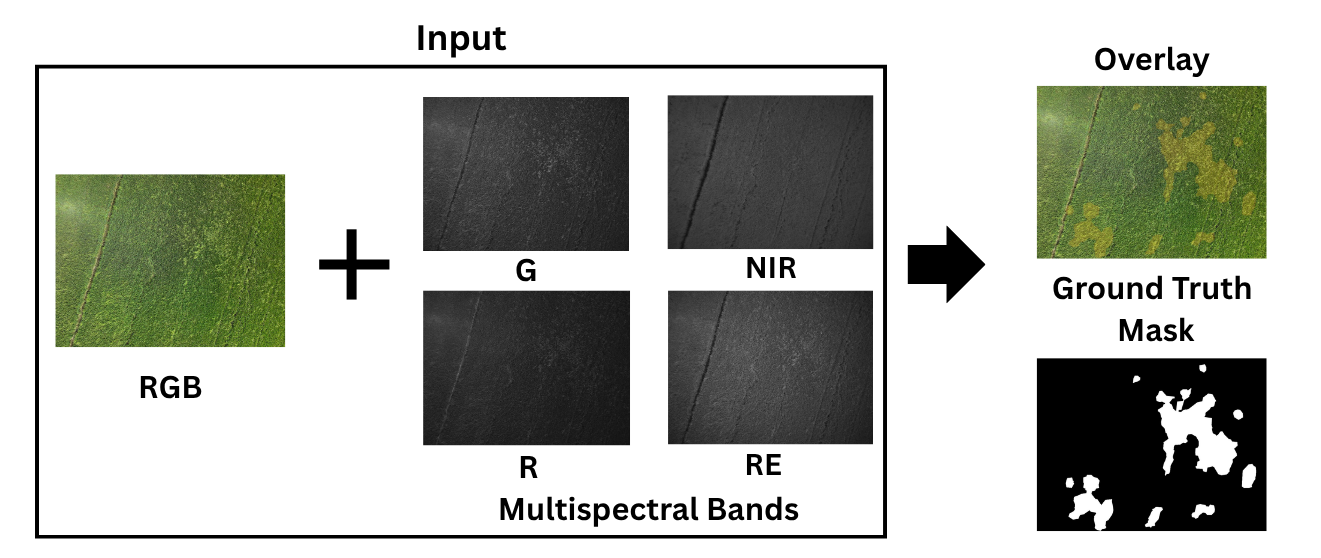
\includegraphics[width=\linewidth]{Images/Dataset_Sample3.png}
\caption{Overview of the WeedyRice-RGBMS-DB dataset structure. Each sample consists of an RGB image and corresponding multispectral bands, including Green (G), Near-Infrared (NIR), Red (R), and Red Edge (RE) channels. The dataset additionally provides overlay visualizations and pixel-wise ground truth masks for weed segmentation.}
\label{fig:dataset_sample}
\end{figure*}

\subsection{Dataset Description}
The experiments are conducted on the Weedy Rice RGB-Multispectral (WeedyRice-RGBMS-DB) dataset \cite{nguyen2025dataset}, a UAV-based multimodal dataset designed for weedy rice segmentation in agricultural fields. The dataset was collected using a DJI M3M UAV over rice fields in An Giang Province, Vietnam, and is geo-referenced in the WGS 84/UTM Zone 48N coordinate system. It includes RGB images, multispectral images, binary segmentation masks, overlay visualizations, and associated metadata. A sample dataset structure is shown in Fig~\ref{fig:dataset_sample}. The dataset consists of a total of 734 samples, divided into training, validation, and test splits. Each sample contains an RGB image (3 channels) along with multispectral bands, namely Green (G), Red (R), Red Edge (RE), and Near-Infrared (NIR), and a corresponding pixel-wise binary ground-truth mask. All images are resized to $512 \times 512$ resolution for uniform processing. For multispectral experiments, the model adopts a dual-branch architecture where the RGB encoder receives a 3-channel RGB image and the multispectral encoder receives a 6-channel input composed of 4 spectral bands and 2 vegetation indices.

In terms of dataset composition, the RGB subset contains 734 images of resolution $1280 \times 960$, while the multispectral subset includes 2936 spatially aligned band images (four bands per RGB image). The ground-truth masks (734 images) provide pixel-level annotations for weedy rice detection, where pixel value 255 denotes weedy rice and 0 represents the background. Overlay images are provided for qualitative evaluation. Metadata files include acquisition details such as GPS coordinates, altitude, timestamp, sensor type, and filename mappings to ensure data consistency. The dataset is divided into 438 training images, 148 validation images, and 148 testing images by the dataset authors. 
% \subsection{Experimental Setting}
% To make the comparisons fair, all the models are implemented in Pytorch and trained under identical experimental settings. The training process for all models used both RGB and multispectral images and was performed on a 13th Gen Intel(R) Core i9-13900K (3.00 GHz) processor, an NVIDIA RTX A5000 GPU with 24 GB memory, 128 GB RAM, 1 TB SSD, and 2 TB HDD. The Software environment was Windows 11 Pro, Python 3.10.20, and CUDA 12.4 for accelerated training. We used the same data split as in Table~\ref{tab:dataset_stats} for training, validation and testing. We considered all the evaluation metrics discussed in Section~\ref{evaluation_metrics} for the performance assessment.




\subsection{Evaluation Metrics}
\label{evaluation_metrics}

To quantify crop-weed segmentation result, performance is reported across five key metrics: Accuracy, Precision, Recall, IoU, and Dice score.
\begin{equation}
\text{Accuracy} = \frac{TP + TN}{TP + TN + FP + FN}
\end{equation}
\begin{equation}
\text{Precision} = \frac{TP}{TP + FP}
\end{equation}
\begin{equation}
\text{Recall} = \frac{TP}{TP + FN}
\end{equation}
\begin{equation}
\text{IoU} = \frac{TP}{TP + FP + FN}
\end{equation}
\begin{equation}
\text{Dice} = \frac{2TP}{2TP + FP + FN}
\end{equation}
where $TP$, $TN$, $FP$, and $FN$ denote true positives, true negatives, false positives, and false negatives, respectively.


% \begin{table*}[t]
% \centering
% \caption{Comparison of the proposed method with CNN-based, transformer-based, and hybrid segmentation approaches. Results are reported as mean $\pm$ standard deviation (in \%).}
% \label{tab:comparison}
% \begin{tabular}{lccccc}
% \hline
% \textbf{Method} & \textbf{Accuracy (\%)} & \textbf{Precision (\%)} & \textbf{Recall (\%)} & \textbf{IoU (\%)} & \textbf{Dice (\%)} \\
% \hline

% \textbf{CNN-based} \\

% U-Net \cite{ronneberger2015unet} 
% & 84.17 $\pm$ 0.40 
% & 69.28 $\pm$ 0.54 
% & 76.54 $\pm$ 1.94 
% & 56.46 $\pm$ 1.28 
% & 69.98 $\pm$ 1.20 \\

% \hline
% \textbf{Transformer-based} \\

% Vision Transformer (ViT) \cite{dosovitskiy2021vit} 
% & 83.84 $\pm$ 0.25 
% & 65.03 $\pm$ 0.99 
% & 74.33 $\pm$ 1.30 
% & 54.43 $\pm$ 0.23 
% & 68.32 $\pm$ 0.23 \\

% SegFormer \cite{xie2021segformer} 
% & 87.73 $\pm$ 0.11 
% & 74.47 $\pm$ 1.04 
% & 71.58 $\pm$ 0.72 
% & 58.45 $\pm$ 0.33 
% & 71.74 $\pm$ 0.41 \\

% \hline
% \textbf{Hybrid (CNN + Transformer)} \\

% TransUNet \cite{chen2021transunet} 
% & 88.36 $\pm$ 0.52 
% & 74.39 $\pm$ 1.81 
% & 80.59 $\pm$ 1.53 
% & 63.55 $\pm$ 0.65 
% & 76.30 $\pm$ 0.55 \\

% Swin-UNet (Hybrid Swin Transformer) \cite{liu2021swin} 
% & 88.35 $\pm$ 0.16 
% & 76.92 $\pm$ 0.39 
% & 75.92 $\pm$ 1.41 
% & 62.16 $\pm$ 0.80 
% & 75.11 $\pm$ 0.74 \\

% CNN + Transformer + Contrastive \cite{chen2020simple} 
% & 89.95 $\pm$ 0.27 
% & 77.10 $\pm$ 1.20 
% & 83.01 $\pm$ 1.18 
% & 67.28 $\pm$ 0.49 
% & 79.37 $\pm$ 0.38 \\

% \hline
% \textbf{CNN (Advanced Baseline)} \\

% DeepLabV3+ \cite{chen2018deeplab} 
% & 90.83 $\pm$ 0.22 
% & 79.12 $\pm$ 1.37 
% & 82.24 $\pm$ 2.06 
% & 68.45 $\pm$ 0.31 
% & 80.22 $\pm$ 0.30 \\

% \hline
% \textbf{Proposed Method} \\

% \textbf{MAViF-Net} 
% & \textbf{91.33 $\pm$ 0.07} 
% & \textbf{80.63 $\pm$ 1.19} 
% & \textbf{83.10 $\pm$ 1.32} 
% & \textbf{70.00 $\pm$ 0.14} 
% & \textbf{81.46 $\pm$ 0.11} \\

% \hline
% \end{tabular}
% \end{table*}

% \subsection{Quantitative Results}

% All competing methods are re-implemented and trained under the same experimental settings, including identical data splits, input resolution, optimizer, and training schedule, to ensure a fair comparison. 

% \subsection{Experimental Protocol}

% Each experiment is repeated five times with different random seeds to ensure robustness and statistical reliability. The final performance is reported on the test set as mean $\pm$ standard deviation.


% \subsection{Comparison with State-of-the-Art Methods}

% To show the effectiveness of our proposed framework, we conducted extensive experiments and comparisons with a diverse set of state-of-the-art (SOTA) segmentation models. These comparative models covering CNN-based architectures, pure transformer-based models, and hybrid CNN-Transformer frameworks. The compared  methods include U-Net \cite{ronneberger2015unet}, Vision Transformer (ViT) \cite{dosovitskiy2021vit}, SegFormer \cite{xie2021segformer}, TransUNet \cite{chen2021transunet}, Swin Transformer-based architectures \cite{liu2021swin}, and DeepLabV3+ \cite{chen2018deeplab}. Further recent hybrid strategies incorporating contrastive learning and multimodal feature integration are included for comparison.

% The quantitative results in terms of Dice Score, Intersection over Union (IoU), Recall, Precision, Accuracy are reported in Table ~\ref{tab:comparison}. All the results are presented as mean $\pm$ standard deviation over five runs. The results reported in the table clearly show that the performance of the models improves as the representation capability and complexity of the model increases from CNN based to transformer-based and finally to hybrid based.

% Simple CNN-based architecture such as U-Net is a strong baseline model for segmentation kind of tasks. However, its receptive filed limits their capability to capture long range dependencies in complicated agriculture environment, resulting lower IoU and Dice scores compared to advance models architectures.

% As Transformer-based models such as ViT and SegFormer consider self-attention mechanism, they are capable of capturing long-range dependency. However, still faces challenges in local information, which is crucial for discriminating crop-weed segmentation tasks, resulting degradation in performance. The segFromer's performance is somewhat good compared to ViT as it is specifically designed for segmentation tasks. While segFormers performance improves over U-Net in term of accuracy Precision, IoU, and Dice score, but their performance is underperformed compared  to hybrid( CNN+Transformers) based architectures.

% Hybrid based models such as TransUNet, and Swin-UNet overcome these challenges by combining both convolutions layers and transformer blocks for preserving both local and global dependencies. This combined model lead to significant improvement in Dice, IoU, Recall, Precision, Accuracy. Further we observed improvement in performance by integrating contrastive loss to these hybrid models. Integrating contrastive loss ensures the better discrimination in embedding space and  gives complementary information which is very useful in scenarios with overlapping vegetation and complicated environment, resulting improvement in all the performance measures.

% Compared to all other SoTA approaches, our proposed framework outperforms in term of all the performance measures. More specifically, The proposed framework achieves 70.00\% IoU and 81.46\% Dice score, outperforming the advanced baseline DeepLabV3+ by 2.26\% and 1.54\%, respectively. Even though the improvement is numerically moderate, but consistent across all the performance measures, and is also supported by low SD, highlighting stable performance across different run.

% It can be seen that the proposed algorithm gives the maximum value of recall (83.12), which is an indication of its efficiency in minimizing false negatives. This is especially critical for agriculture weed segmentation because missed regions in the weeds could affect future decisions. Though the precision is slightly inferior to that of DeepLabV3+, the combined effect of precision and recall produces better results in terms of image segmentation measures, such as Intersection-over-Union (IoU) and Dice Score.

% In conclusion, these findings demonstrate that the proposed framework successfully leverages the capability of CNNs to maintain local features, the attention mechanism to maintain global information, and the use of multiple models and late fusion techniques for better differentiation of features.
\section{Results and Discussion}
To evaluate the effectiveness of the proposed framework, extensive experiments are conducted against a diverse set of state-of-the-art (SOTA) models, including CNN-based, transformer-based, and hybrid CNN--Transformer architectures. The compared methods include U-Net \cite{ronneberger2015unet}, PSPNet \cite{zhao2017pyramid}, U-Net++ \cite{zhou2018unet++}, DenseUNet \cite{mu2023densenet}, DeepLabV3 \cite{chen2018Deeplabv3plus}, Vision Transformer (ViT) \cite{dosovitskiy2021vit}, SegFormer \cite{xie2021segformer}, Swin Transformer-based models \cite{liu2021swin}, CRF-UNet \cite{sahin2023segmentation}, and hybrid CNN-Transformer, frameworks \cite{guo2025cnn_transformer}.

Table~\ref{tab:results} presents the quantitative results, where all metrics are reported as mean $\pm$ standard deviation (in \%) over five independent runs, each with a different seed value. The results show a gradual performance improvement from conventional CNN-based methods to transformer-based and hybrid architectures, highlighting the importance of adaptively combining local spatial information with global contextual representations.

CNN-based architectures such as U-Net provide a strong baseline, achieving 89.68\% accuracy and a 68.75\% IoU. These models capture local spatial patterns important for distinguishing crop and weed textures. However, their receptive field is limited, which restricts their ability to model long-range contextual dependencies in complex agricultural scenes. Advanced CNN architectures attempt to address this limitation through improved feature aggregation strategies. PSPNet learns the context information of multiple scales by pyramid pooling, U-Net++ improves the feature propagation by nested skip connections, and DenseUNet applies dense connectivity to reuse features more effectively. Thus, DenseUNet achieves better performance than other conventional CNN-based methods with an IoU score of 70.67\%, while Unet++ also provides competitive performance through improved feature propagation.

Transformer-based approaches such as ViT and SegFormer use self-attention mechanisms to better capture global dependencies. However, the local inductive bias of pure transformer architectures is weaker, which limits their ability to preserve the fine spatial details needed for accurate boundary localization. As a result, ViT achieves only 56.08\% IoU, while SegFormer improves the performance to 59.04\% IoU and 73.13\% Dice through hierarchical feature representations. Nevertheless, these models still underperform compared to stronger CNN-based approaches such as DenseUNet. Hybrid CNN-Transformer architectures combine the strengths of both paradigms by jointly learning local texture information and global contextual relationships. This leads to improved segmentation performance, with CNN+Transformer and Swin Transformer achieving IoU scores of 63.55\% and 75.43\%, respectively. However, their performance remains limited due to insufficient exploitation of multimodal spectral information and the absence of effective feature fusion mechanisms.
\begin{figure*}[t]
\centering
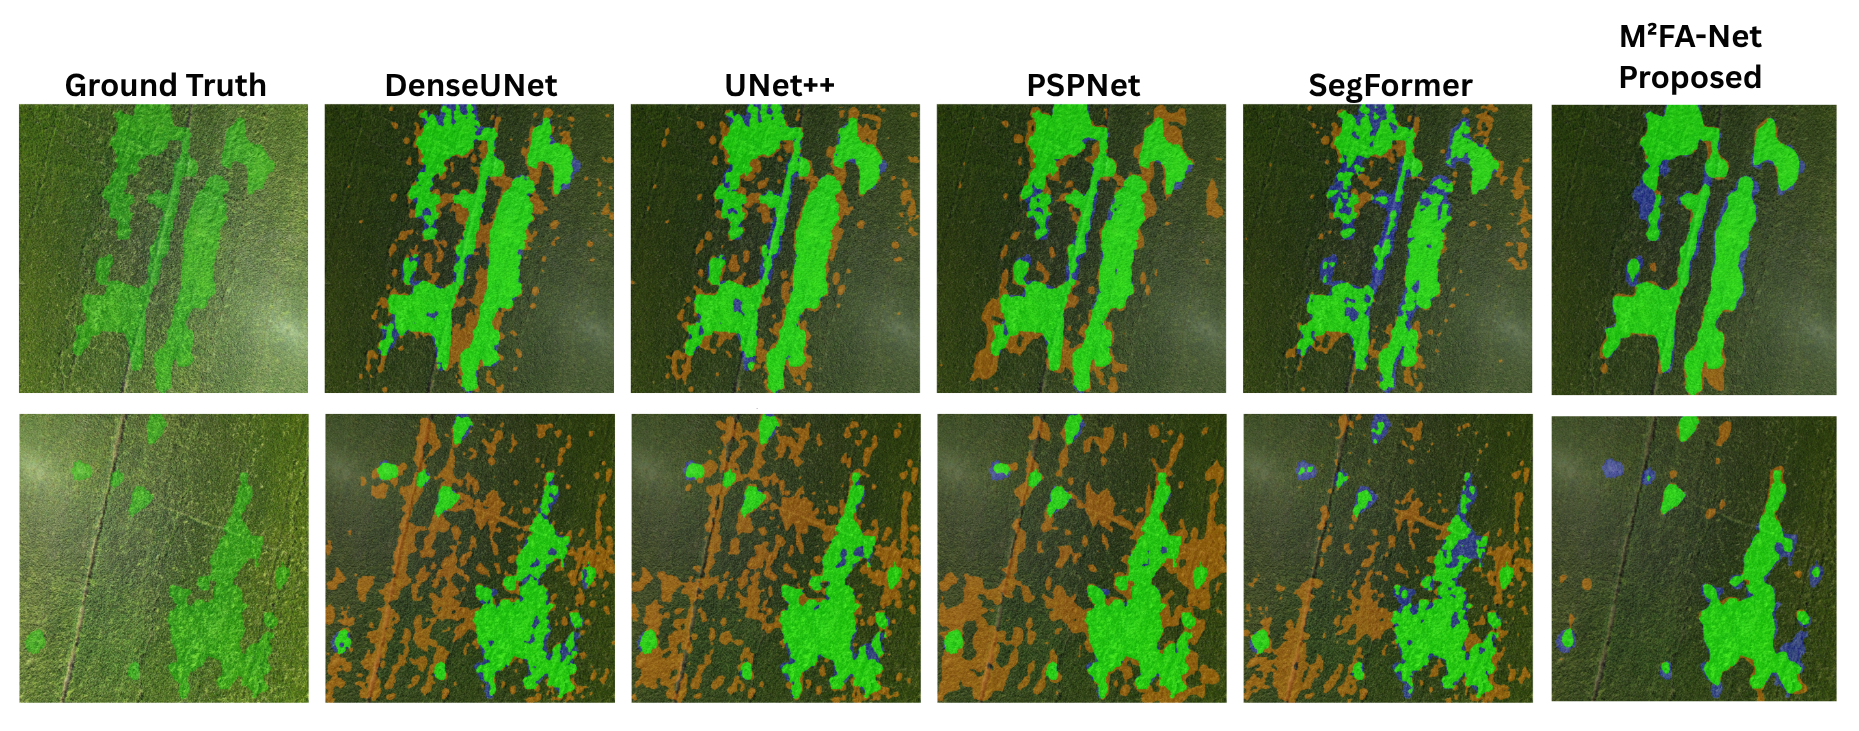
\includegraphics[width=\linewidth]{Images/Comparison_new.png}
\caption{Qualitative comparison of crop--weed segmentation results produced by different state-of-the-art models on representative field samples. The proposed $M^2$FA-Net generates cleaner segmentation masks with improved structural consistency, sharper boundary localization, and significantly fewer segmentation artifacts compared to DenseUNet, U-Net++, PSPNet, and SegFormer, particularly in dense vegetation and sparse weed regions.}
\label{fig:comparison}
\end{figure*}

\begin{table*}[t]

\setlength{\tabcolsep}{4pt}
\caption{Performance comparison of different models for crop--weed segmentation. Results are reported as mean $\pm$ standard deviation (in \%).}
\label{tab:results}
\resizebox{\textwidth}{!}{%
\begin{tabular}{lccccc}
\hline
\textbf{Method} & \textbf{Accuracy (\%)} & \textbf{Precision (\%)} & \textbf{Recall (\%)} & \textbf{IoU (\%)} & \textbf{Dice (\%)} \\
\hline

U-Net \cite{ronneberger2015unet}
& 89.68 $\pm$ 0.40 
& 82.18 $\pm$ 2.59 
& 80.44 $\pm$ 2.36 
& 68.75 $\pm$ 0.46 
& 80.97 $\pm$ 0.33 \\

Transformer (ViT) \cite{dosovitskiy2021vit}
& 82.48 $\pm$ 0.57 
& 66.99 $\pm$ 1.94 
& 76.78 $\pm$ 2.45 
& 56.08 $\pm$ 0.20
& 70.87 $\pm$ 0.19 \\

HRNet \cite{sun2019high}
& 81.67 $\pm$ 0.62 
& 63.48 $\pm$ 1.88 
& 73.21 $\pm$ 2.76 
& 52.72 $\pm$ 0.41 
& 67.36 $\pm$ 0.43 \\

PSPNet \cite{zhao2017pyramid}
& 89.87 $\pm$ 0.33 
& 79.82 $\pm$ 1.35 
& 83.27 $\pm$ 1.61 
& 69.34 $\pm$ 0.59 
& 81.36 $\pm$ 0.40 \\



DeepLabV3 \cite{chen2018Deeplabv3plus}
& 88.89 $\pm$ 0.24 
& 79.81 $\pm$ 2.11 
& 80.23 $\pm$ 2.43 
& 66.95 $\pm$ 0.54 
& 79.62 $\pm$ 0.41 \\


CRF-U-Net \cite{sahin2023segmentation}
& 88.91 $\pm$ 0.89 
& 80.11 $\pm$ 2.01 
& 79.76 $\pm$ 3.86 
& 66.82 $\pm$ 2.55 
& 79.54 $\pm$ 1.93 \\

SegFormer \cite{xie2021segformer}
& 86.04 $\pm$ 0.63 
& 78.65 $\pm$ 2.23 
& 70.58 $\pm$ 3.54 
& 59.04 $\pm$ 1.87 
& 73.13 $\pm$ 1.56 \\

CNN + Transformer \cite{guo2025cnn_transformer}
& 88.36 $\pm$ 0.52 
& 74.39 $\pm$ 1.81 
& 80.59 $\pm$ 1.53 
& 63.55 $\pm$ 0.65 
& 76.30 $\pm$ 0.55 \\

Swin Transformer \cite{liu2021swin}
& 90.58 $\pm$ 0.39 
& 85.99 $\pm$ 2.19 
& 86.13 $\pm$ 2.83 
& 75.43 $\pm$ 1.03 
& 85.99 $\pm$ 0.67 \\

U-Net++ \cite{zhou2018unet++}
& 90.41 $\pm$ 0.13 
& 80.28 $\pm$ 2.16 
& 78.26 $\pm$ 1.81 
& 66.39 $\pm$ 0.27 
& 78.56 $\pm$ 0.22 \\

DenseUNet \cite{mu2023densenet}
& 90.75 $\pm$ 0.26
& 83.77 $\pm$ 2.88 
& 81.38 $\pm$ 2.78 
& 70.67 $\pm$ 0.31 
& 82.27 $\pm$ 0.23 \\

\textbf{$M^2$FA-Net(Proposed)}
& \textbf{94.06 $\pm$ 0.07} 
& \textbf{90.72 $\pm$ 0.69}
& \textbf{87.82 $\pm$ 0.84} 
& \textbf{80.79 $\pm$ 0.24} 
& \textbf{89.21 $\pm$ 0.15} \\

\hline
\end{tabular}
}
\end{table*}



DeepLab-based architectures further improve segmentation performance through multi-scale contextual aggregation using dilated convolutions. DeepLabV3 achieves 66.95\% IoU and 79.62\% Dice, outperforming several CNN and transformer-based approaches. This demonstrates the effectiveness of multi-scale feature extraction and contextual learning for agricultural segmentation tasks. However, convolution-only approaches still face challenges in modeling complex multimodal feature interactions. 
In contrast, the proposed $M^2$FA-Net achieves the best performance across all evaluation metrics, obtaining 94.06\% accuracy, 90.72\% precision, 87.82\% recall, 80.79\% IoU, and 89.21\% Dice score. Compared to the strongest baseline methods, $M^2$FA-Net improves IoU by 10.12\% over DenseUNet and Dice score by 10.65\% over U-Net++. The proposed framework also outperforms DeepLabV3 by 13.84\% in IoU and 9.59\% in Dice score. In addition, $M^2$FA-Net has the highest recall among all methods, indicating the reduction of false negatives and improvement of the weed detection capability, which is important for precision agriculture applications.


As shown in the first sample in Fig.~\ref{fig:comparison}, most baseline methods fail to distinguish weeds from cultivated rice due to the strong visual similarity in terms of texture and color. PSPNet shows aggressive over-segmentation, and SegFormer produces sparse false activations in dense vegetation regions. The proposed $M^2$FA-Net, on the other hand, produces smoother and more coherent segmentation masks, with sharper boundaries and substantially fewer misclassification errors. The second sample shows a more difficult situation with scarce and dispersed weed regions. Existing approaches are not able to model thin weed structures accurately and tend to classify surrounding background areas as weeds, leading to noisy predictions and more false negatives. In contrast, the proposed $M^2$FA-Net can accurately detect both large and small weed regions with good boundary preservation and low background noise. 
\subsection{Ablation Study}
To evaluate the effectiveness of each component in the proposed $M^2$FA-Net framework, an ablation study is conducted by systematically removing individual modules, including multi-level fusion, CBAM attention, deep supervision, warmup scheduling, and data augmentation, and is given in Table~\ref{tab:ablation}. For improved interpretability, the corresponding IoU and Dice
trends are additionally visualized in Fig.~\ref{fig:iou}, while
Fig.~\ref{fig:component_contribution} summarizes the relative
contribution of each architectural component.

As observed in Fig.~\ref{fig:iou}, the complete $M^2$FA-Net consistently achieves the highest IoU and Dice scores, while removing any individual component leads to a performance decline. The largest degradation occurs when multi-level fusion is removed, highlighting its importance within the proposed framework. Fig.~\ref{fig:component_contribution} further summarizes the relative contribution of each component. Multi-level fusion provides the largest performance gain, followed by deep supervision and CBAM attention, indicating that effective multimodal feature integration and attention-guided refinement are the primary contributors to the performance improvements. As observed in Fig.~\ref{fig:iou}, the full $M^2$FA-Net consistently yields the highest IoU and Dice scores, while the removal of any individual module causes a substantial performance decline. The largest drop is observed when multi-level fusion is removed, highlighting its central role in integrating complementary spatial and spectral information.
\begin{table*}[t]
\centering
\caption{Ablation Study on the Impact of Multispectral Data, CBAM Attention, and Vegetation Indices (NDVI and NDRE). Results are reported as mean $\pm$ standard deviation (in \%).}
\label{tab:ablation}
\resizebox{\textwidth}{!}{%

\begin{tabular}{lccccc}
\hline
\textbf{Method} & \textbf{Accuracy (\%)} & \textbf{Precision (\%)} & \textbf{Recall (\%)} & \textbf{IoU (\%)} & \textbf{Dice (\%)} \\
\hline

Baseline (Early Fusion) 
& 92.75 $\pm$ 0.09
& 90.28 $\pm$ 0.42
& 82.98 $\pm$ 0.43 
& 76.48 $\pm$ 0.25 
& 86.41 $\pm$ 0.15 \\

No Multi-Level Fusion
& 92.86 $\pm$ 0.09 
& 90.81 $\pm$ 0.56 
& 82.80 $\pm$ 0.92 
& 76.68 $\pm$ 0.42 
& 86.55 $\pm$ 0.28 \\

No CBAM Attention 
& 93.10 $\pm$ 0.11
& 90.61 $\pm$ 0.80 
& 84.10 $\pm$ 0.98
& 77.62 $\pm$ 0.38
& 87.18 $\pm$ 0.25 \\

No Deep Supervision  
& 93.06 $\pm$ 0.14 
& 90.95 $\pm$ 0.67 
& 83.36 $\pm$ 0.99
& 77.24 $\pm$ 0.51 
& 86.92 $\pm$ 0.34 \\

No Warmup Scheduler
& 92.78 $\pm$ 0.40
& 90.92 $\pm$ 1.80
& 83.10 $\pm$ 3.08
& 76.90 $\pm$ 1.38 
& 86.72 $\pm$ 0.91 \\

No Augmentation   
& 93.26 $\pm$ 0.08 
& 90.60 $\pm$ 0.28
& 84.78 $\pm$ 0.43 
& 78.18 $\pm$ 0.24
& 87.55 $\pm$ 0.15 \\

\textbf{\boldmath$M^2$FA-Net (proposed)}
& \textbf{94.06 $\pm$ 0.07} 
& \textbf{90.72 $\pm$ 0.69} 
& \textbf{87.82 $\pm$ 0.84} 
& \textbf{80.79 $\pm$ 0.24} 
& \textbf{89.21 $\pm$ 0.15} \\

\hline
\end{tabular}
}
\end{table*}
\begin{figure}[t]
    \centering
    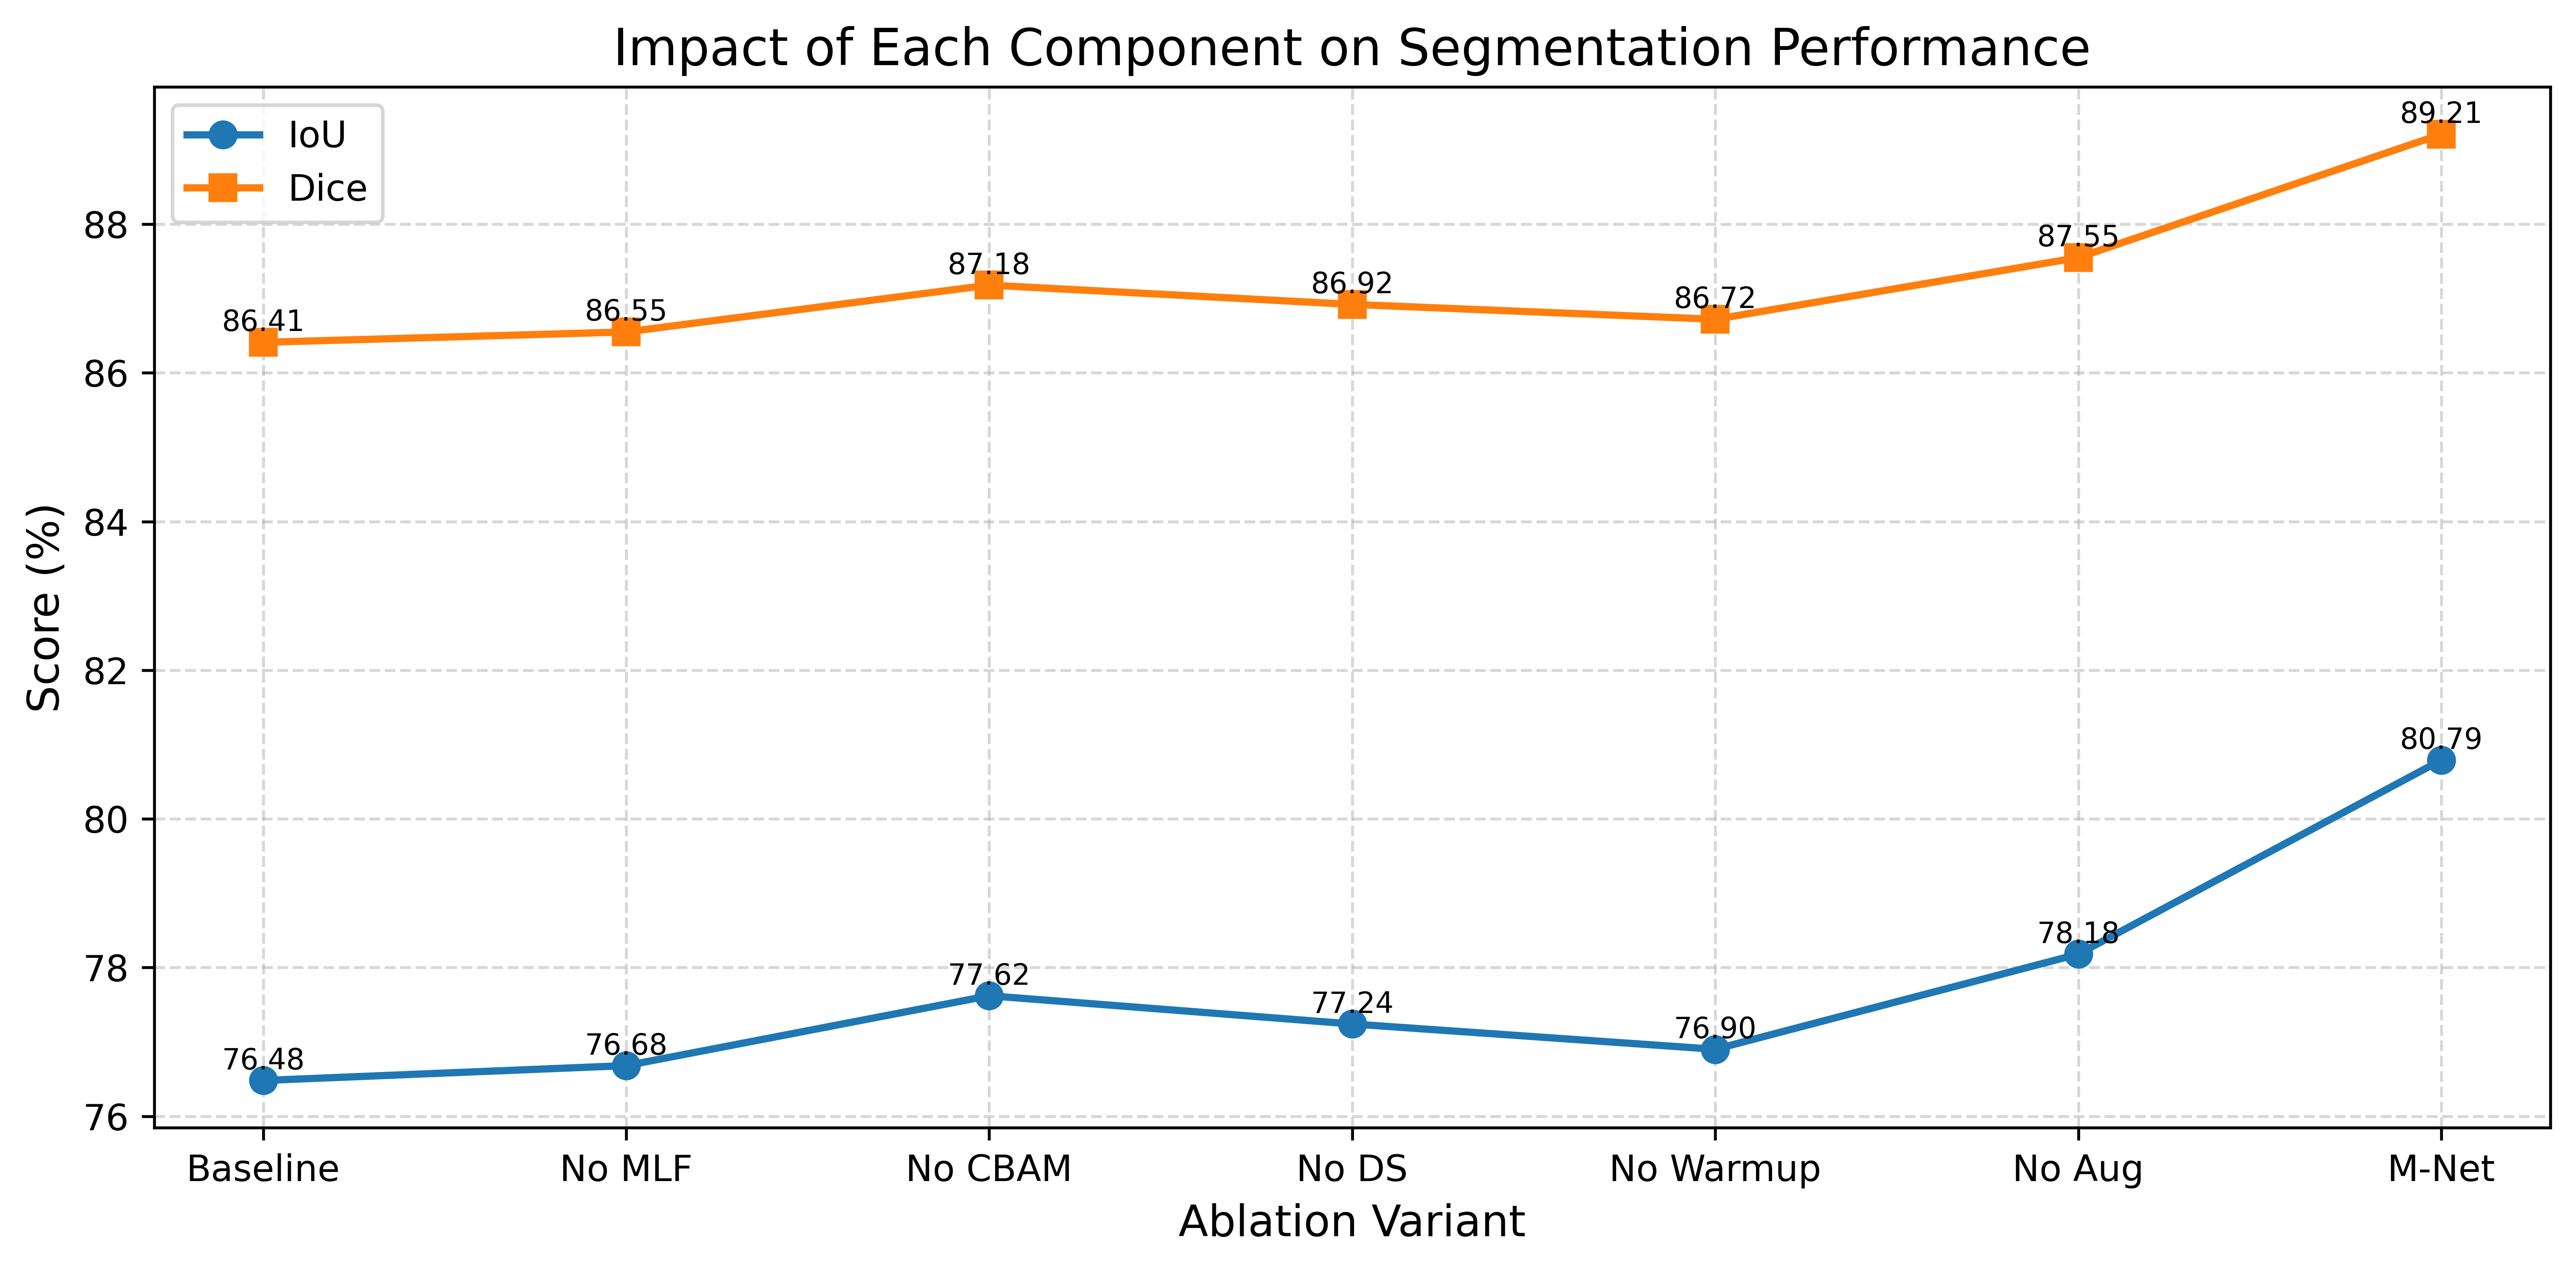
\includegraphics[width=12cm]{Images/ablation_iou_dice (2).png}
    \caption{Effect of removing individual components from the proposed $M^2$FA-Net framework. The complete model achieves the highest IoU and Dice scores, demonstrating the complementary contributions of multi-level fusion (MLF), CBAM attention, deep supervision (DS), warmup scheduling, and data augmentation.}
    \label{fig:iou}
\end{figure}
\begin{figure}[t]
    \centering
    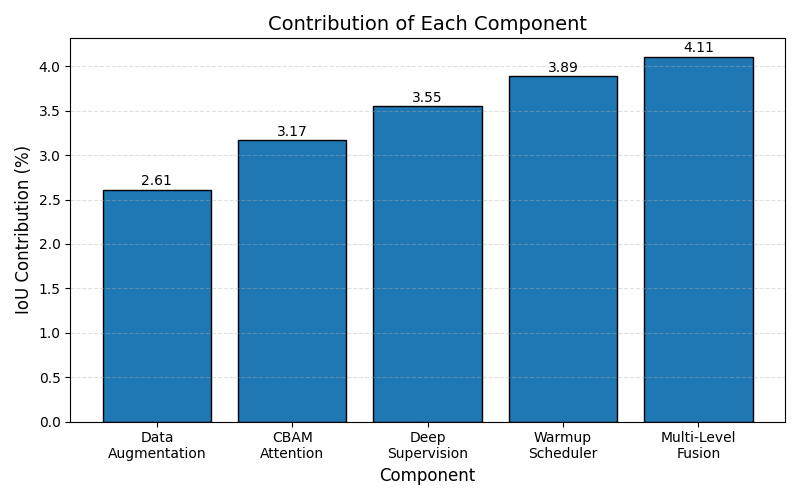
\includegraphics[width=12cm]{Images/contribution.png}
    \caption{Relative IoU contribution of major components in the proposed $M^2$FA-Net framework. Multi-level fusion provides the largest performance gain, followed by deep supervision, CBAM attention, warmup scheduling, and data augmentation, highlighting the effectiveness of the integrated design.}
    \label{fig:component_contribution}
\end{figure}
Along with the overall ablation comparison, Fig.~\ref{fig:component_contribution} provides a more detailed look at the relative contribution of each architectural component. Multi-level fusion provides the biggest improvement, followed by deep supervision and CBAM attention. This shows that effective multimodal integration and better feature optimization are key factors in the strong performance of the proposed framework.




\subsection{Computational Complexity Analysis}

To further evaluate the efficiency of the proposed framework, a computational complexity analysis was conducted in terms of the number of parameters, floating point operations (FLOPs), and inference speed measured in frames per second (FPS). All complexity metrics were computed using an input resolution of $512 \times 512$, while FPS was measured using batch size 1 under inference mode using the same hardware configuration described in Section IV.


\begin{table}[h]
\centering
\caption{Computational complexity comparison of different segmentation models in terms of FLOPs and inference speed}
\label{tab:complexity}
\begin{tabular}{lccc}
\hline
Model & FLOPs (G) & Inference Speed\\
\hline
DenseUNet  & 68.60 & 47.00 \\
UNet++  & 148.29 & 40.81 \\
PSPNet  & 19.53 & 280.11 \\
SegFormer  & 6.77 & 194.58 \\
$M^2$FA-Net (Proposed)  & 267.68 & 40.22 \\
\hline
\end{tabular}
\end{table}

\begin{figure}[t]
    \centering
    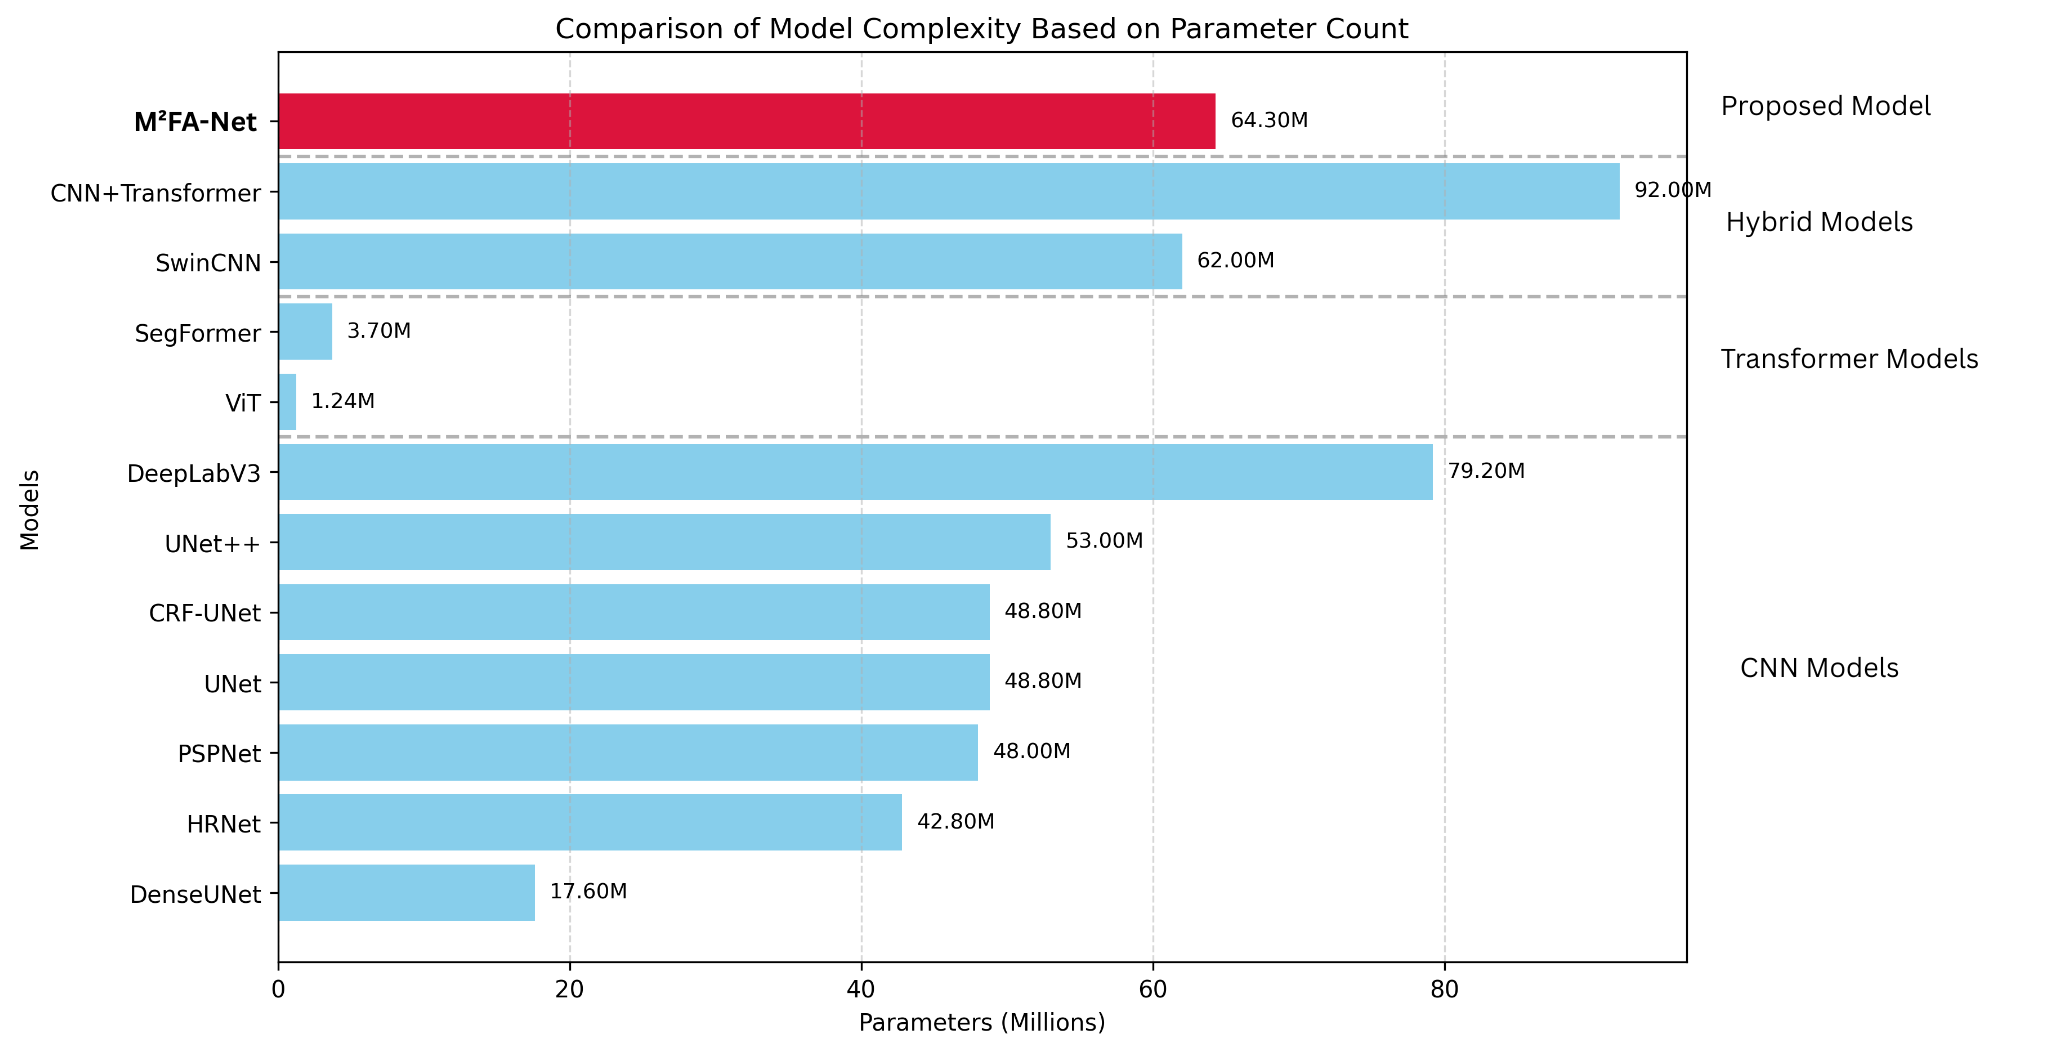
\includegraphics[width=17cm]{Images/parameters.png}
    % Parameter Comparison
\caption{Comparison of model complexity in terms of parameter count across representative CNN-based, transformer-based, hybrid, and proposed architectures. Although $M^2$FA-Net contains more parameters than several baseline models, it remains substantially lighter than some transformer-hybrid frameworks while achieving superior segmentation performance.}
    \label{fig:parameter}
\end{figure}

Table~\ref{tab:complexity} presents the computational complexity comparison of different segmentation models in terms of FLOPs and inference speed. Figure~\ref{fig:parameter} further compares the parameter count of representative segmentation architectures. Although the proposed framework is computationally more demanding than lightweight architectures such as PSPNet and SegFormer, it still maintains competitive inference speed while delivering significantly superior segmentation accuracy. Taking into account substantial improvements in IoU and Dice score, the additional computational cost is justified for precision agriculture applications where segmentation quality is of primary importance. Overall, the proposed $M^2$FA-Net achieves an effective trade-off between computational complexity and segmentation performance.



\subsection{Hyperparameter Sensitivity Analysis}
To further investigate the robustness of the proposed $M^2$FA-Net framework, a series of hyperparameter sensitivity experiments is conducted. Key training parameters, including learning rate, batch size, auxiliary loss weight, warmup epochs, weight decay, and loss function weights, were systematically varied while keeping all other settings unchanged. 
Fig.~\ref{fig:batch_analysis} reveals the effects of batch sizes on segmentation results. The highest performance among the evaluated settings is achieved with a batch size of 8, which was adopted for all subsequent experiments.
Figure~\ref{fig:aux_analysis} shows that increasing the auxiliary loss weight consistently improves segmentation performance. The best performance is achieved at $\lambda=0.7$, which was adopted in the final $M^2$FA-Net framework.
As illustrated in Fig.~\ref{fig:learning_rate}, the results improve significantly when increasing the learning rate from $1\times10^{-5}$, reaching its highest performance at $2\times10^{-4}$, which was selected for the final configuration of the model.



 According to the obtained data, weight decay, warmup epochs, and loss weights have only a slight effect on segmentation efficiency in comparison with the learning rate, batch size, and auxiliary loss weight. For the weight decay parameter within its range from $10^{-5}$ to 1, the difference in val IoU did not exceed 0.5\%. Likewise, variations in the number of warmup epochs between 0 and 5 had only a negligible effect on the framework's performance; the warmup stage of 3 epochs was finally used. Besides, several different loss function weightings for CE, Dice, and Boundary losses led to almost similar results and proved the framework's insensitivity to the specified parameter. Among them, the combination with weights of 0.4 for CE, 0.4 for Dice, and 0.2 for Boundary was recognized as the best one.

\begin{figure*}[t]
\centering
% Top row
\begin{subfigure}[t]{0.48\textwidth}
    \centering
    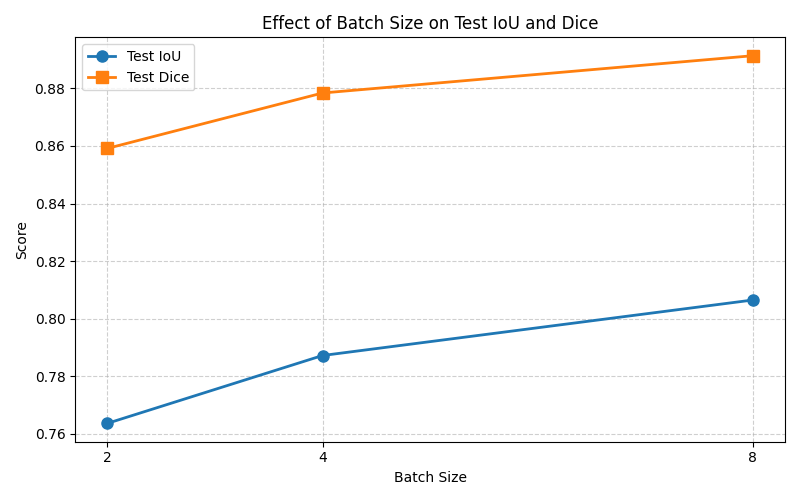
\includegraphics[width=\linewidth]{Images/batchsize_ioudice.png}
    \caption{Effect of batch size on validation IoU and Dice performance.}
    \label{fig:batch_analysis}
\end{subfigure}
\hfill
\begin{subfigure}[t]{0.48\textwidth}
    \centering
    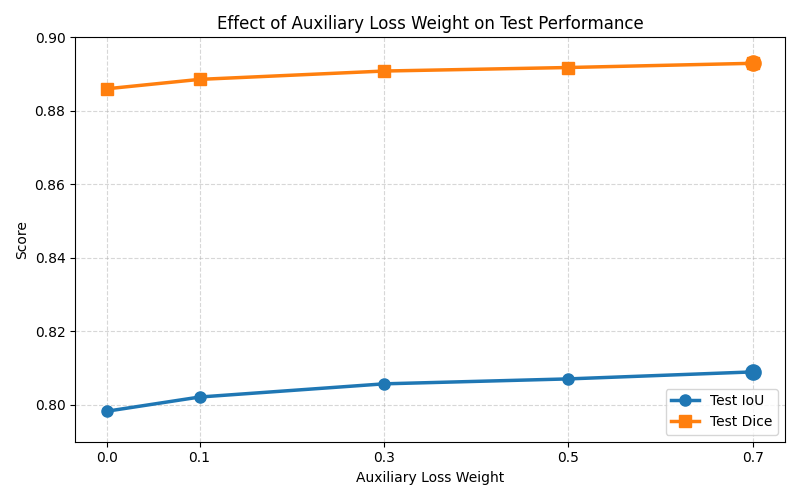
\includegraphics[width=\linewidth]{Images/auxclassifer.png}
    \caption{Effect of auxiliary loss weight ($\lambda$) on validation IoU and Dice performance.}
    \label{fig:aux_analysis}
\end{subfigure}

\vspace{0.5cm}

% Bottom row centered
\begin{subfigure}{0.6\textwidth}
    \centering
    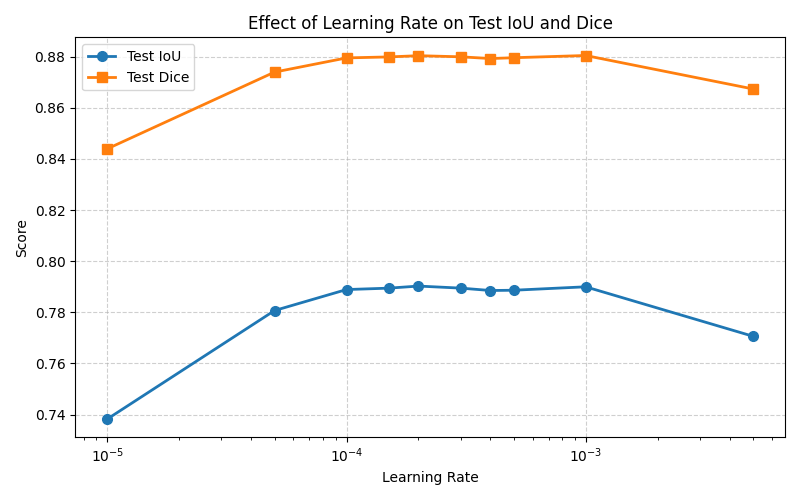
\includegraphics[width=\linewidth]{Images/learningrate_iouudice.png}
    \caption{Impact of learning rate on validation IoU and Dice scores.}
    \label{fig:learning_rate}
\end{subfigure}

\caption{Hyperparameter sensitivity analysis of the proposed $M^2$FA-Net.}
\label{fig:hyperparameter_analysis}

\end{figure*}

To analyze the optimization behavior of the proposed framework,
the evolution of training and validation losses is monitored
throughout the training process. As shown in Fig.~\ref{fig:loss_curves},
both losses decrease steadily across epochs, indicating stable
convergence and effective optimization. Furthermore, the small
gap between the training and validation curves suggests strong
generalization capability and minimal overfitting. In addition to loss convergence, segmentation performance is
tracked using validation IoU and Dice metrics. As illustrated in
Fig.~\ref{fig:iou_dice}, both metrics improve consistently
throughout training before stabilizing during the later epochs.
The steady increase in validation performance confirms the
effectiveness of the proposed training strategy and optimization
settings.

\begin{figure*}[t]
\centering

\begin{subfigure}[t]{0.48\textwidth}
    \centering
    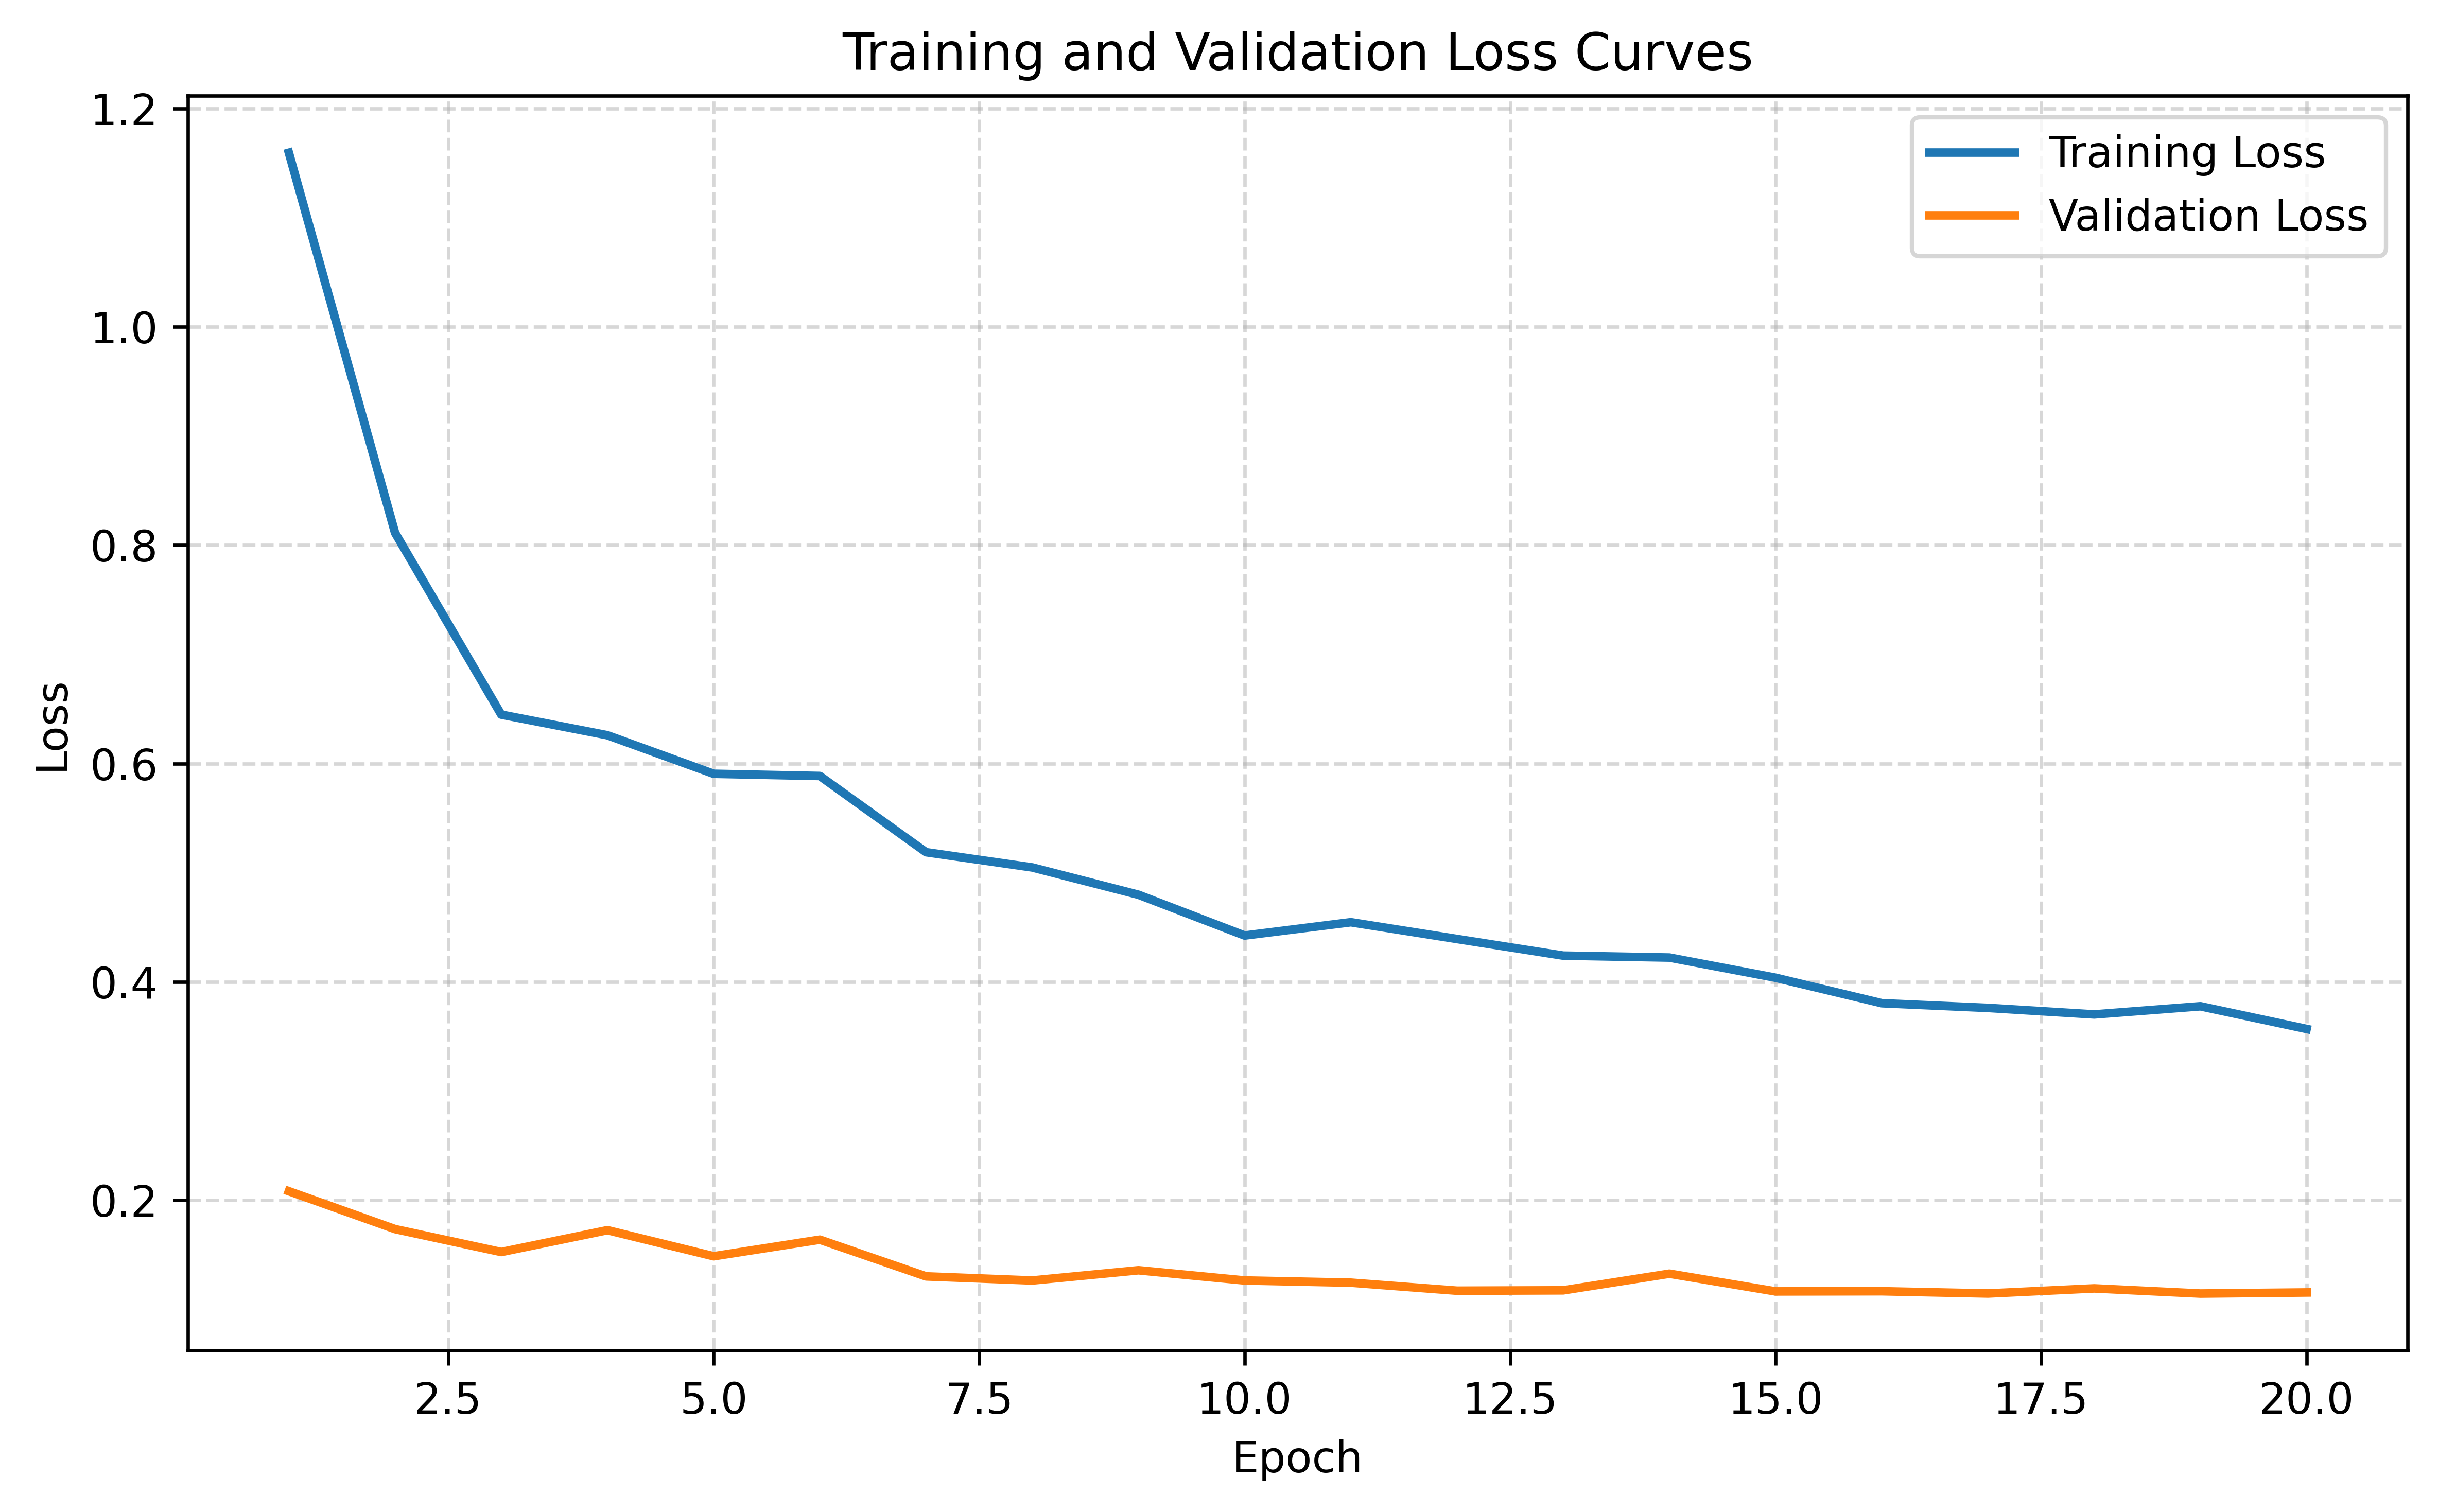
\includegraphics[width=\linewidth]{Images/loss_curves (1).png}
    \caption{Training and validation loss curves of $M^2$FA-Net during optimization. The continuous decline in both losses demonstrates stable convergence with minimal overfitting.}
    \label{fig:loss_curves}
\end{subfigure}
\hfill
\begin{subfigure}[t]{0.48\textwidth}
    \centering
    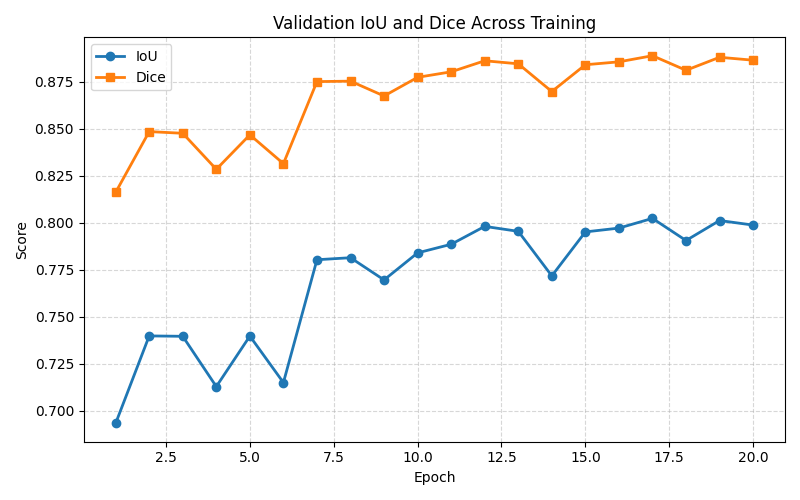
\includegraphics[width=\linewidth]{Images/ioudice_new.png}
    \caption{Validation IoU and Dice scores over 20 training epochs. Both metrics improve consistently and converge to stable values, indicating successful learning and strong generalization.}
    \label{fig:iou_dice}
\end{subfigure}

\caption{Training dynamics of the proposed $M^2$FA-Net. Loss curves demonstrate stable optimization, while IoU and Dice trends indicate progressive improvements in segmentation performance throughout training.}
\label{fig:training_dynamics}

\end{figure*}

\section{Conclusion and Future scope}

In this paper, we proposed $M^2$FA-Net, a multi-level multimodal fusion attention framework for accurate crop–weed segmentation using RGB, multispectral, and vegetation index information. 
The framework integrates dual-stream DeepLabV3 backbones, progressive multi-level feature fusion, CBAM attention modules, deep supervision, and a composite loss function to effectively exploit complementary spatial, spectral, and vegetation-index information. Experimental results demonstrate that $M^2$FA-Net consistently outperforms existing baseline and state-of-the-art methods across all evaluation metrics, achieving 80.79\% IoU and 89.21\% Dice score, while producing sharper boundary localization, improved structural consistency, and reduced segmentation artifacts compared to existing approaches. These findings indicate that $M^2$FA-Net provides an effective and robust solution for crop–weed segmentation and highlights the potential of multimodal learning for advancing intelligent precision agriculture systems.


Research for the future should concentrate on improving
generalization capabilities, scalability, and application aspects of the proposed $M^2$FA-Net framework. Few-shot and low-shot learning can be explored to avoid reliance on the annotation of large volumes of images at the pixel level, whereas
domain adaptation and domain generalization can increase the robustness of the model under varied crop types, geographic regions, sensors, and environmental conditions. Furthermore, the incorporation of agronomical and textual knowledge about the crop through vision-language models could aid in providing additional contextual information for the task of segmentation. The incorporation of foundation models and self-supervised multimodal pretraining also presents a promising direction for leveraging large-scale agricultural data. Furthermore, lightweight variants of $M^2$FA-Net can be developed for real-time deployment on UAVs, edge devices, and autonomous agricultural robots, while extending the framework to multi-class segmentation and spatiotemporal analysis using multi-temporal UAV imagery may further support advanced precision agriculture applications.
\section*{Author Contributions}

Manan Dudeja: Methodology, Software, Data curation, Validation, Writing--original draft.
Rakesh Kumar Sanodiya: Origination and Conceptualization, Data curation, Validation, Supervision, Project administration, Investigation, Writing--review \& editing.
Lekshmi R: Formal analysis, Visualization, Investigation.
Matloob Khushi: Conceptualization, Validation, Supervision, Project administration, Writing--review \& editing.

\section*{Acknowledgment}
We thank the anonymous reviewers for their careful reading and constructive feedback, which helped improve this manuscript.

\section*{Funding}
This work was supported by the
Science and Engineering Research Board (SERB)
under the Core Research Grant Project (File No. 
CRG/2023/001239). 

\section*{Data Availability}

The WeedyRice-RGBMS-DB dataset used in this work is publicly available at: 

https://data.mendeley.com/datasets/vt4s83pxx6/1

\section*{Competing Interests}

The authors declare that they have no competing interests.


\bibliography{sn-bibliography}



\end{document}
